\chapter{Discussion}\label{chap:discussion}

In this section, we are going to discuss the before-presented results of the experiments. We focus hereby only on the results from the Reinforcement Learning section in \chapref{chap:experiments}.

\section{Baseline SAC}


Let's delve into the foundational results of the baseline SAC experiments. We immediately noticed a pronounced correlation between the performance of the SAC algorithm and the number of joints it was trained on. This connection is quite logical, as the effectiveness and computational demands of other inverse kinematics solvers, such as CCD, are intricately linked to the number of joints in the robotic system. This connection beautifully aligns with the runtime complexity analysis portrayed in \figref{fig:expert_dataset/runtime_complexity}.


\begin{figure}
    \begin{center}
        \subfloat[$N = 2$]{
            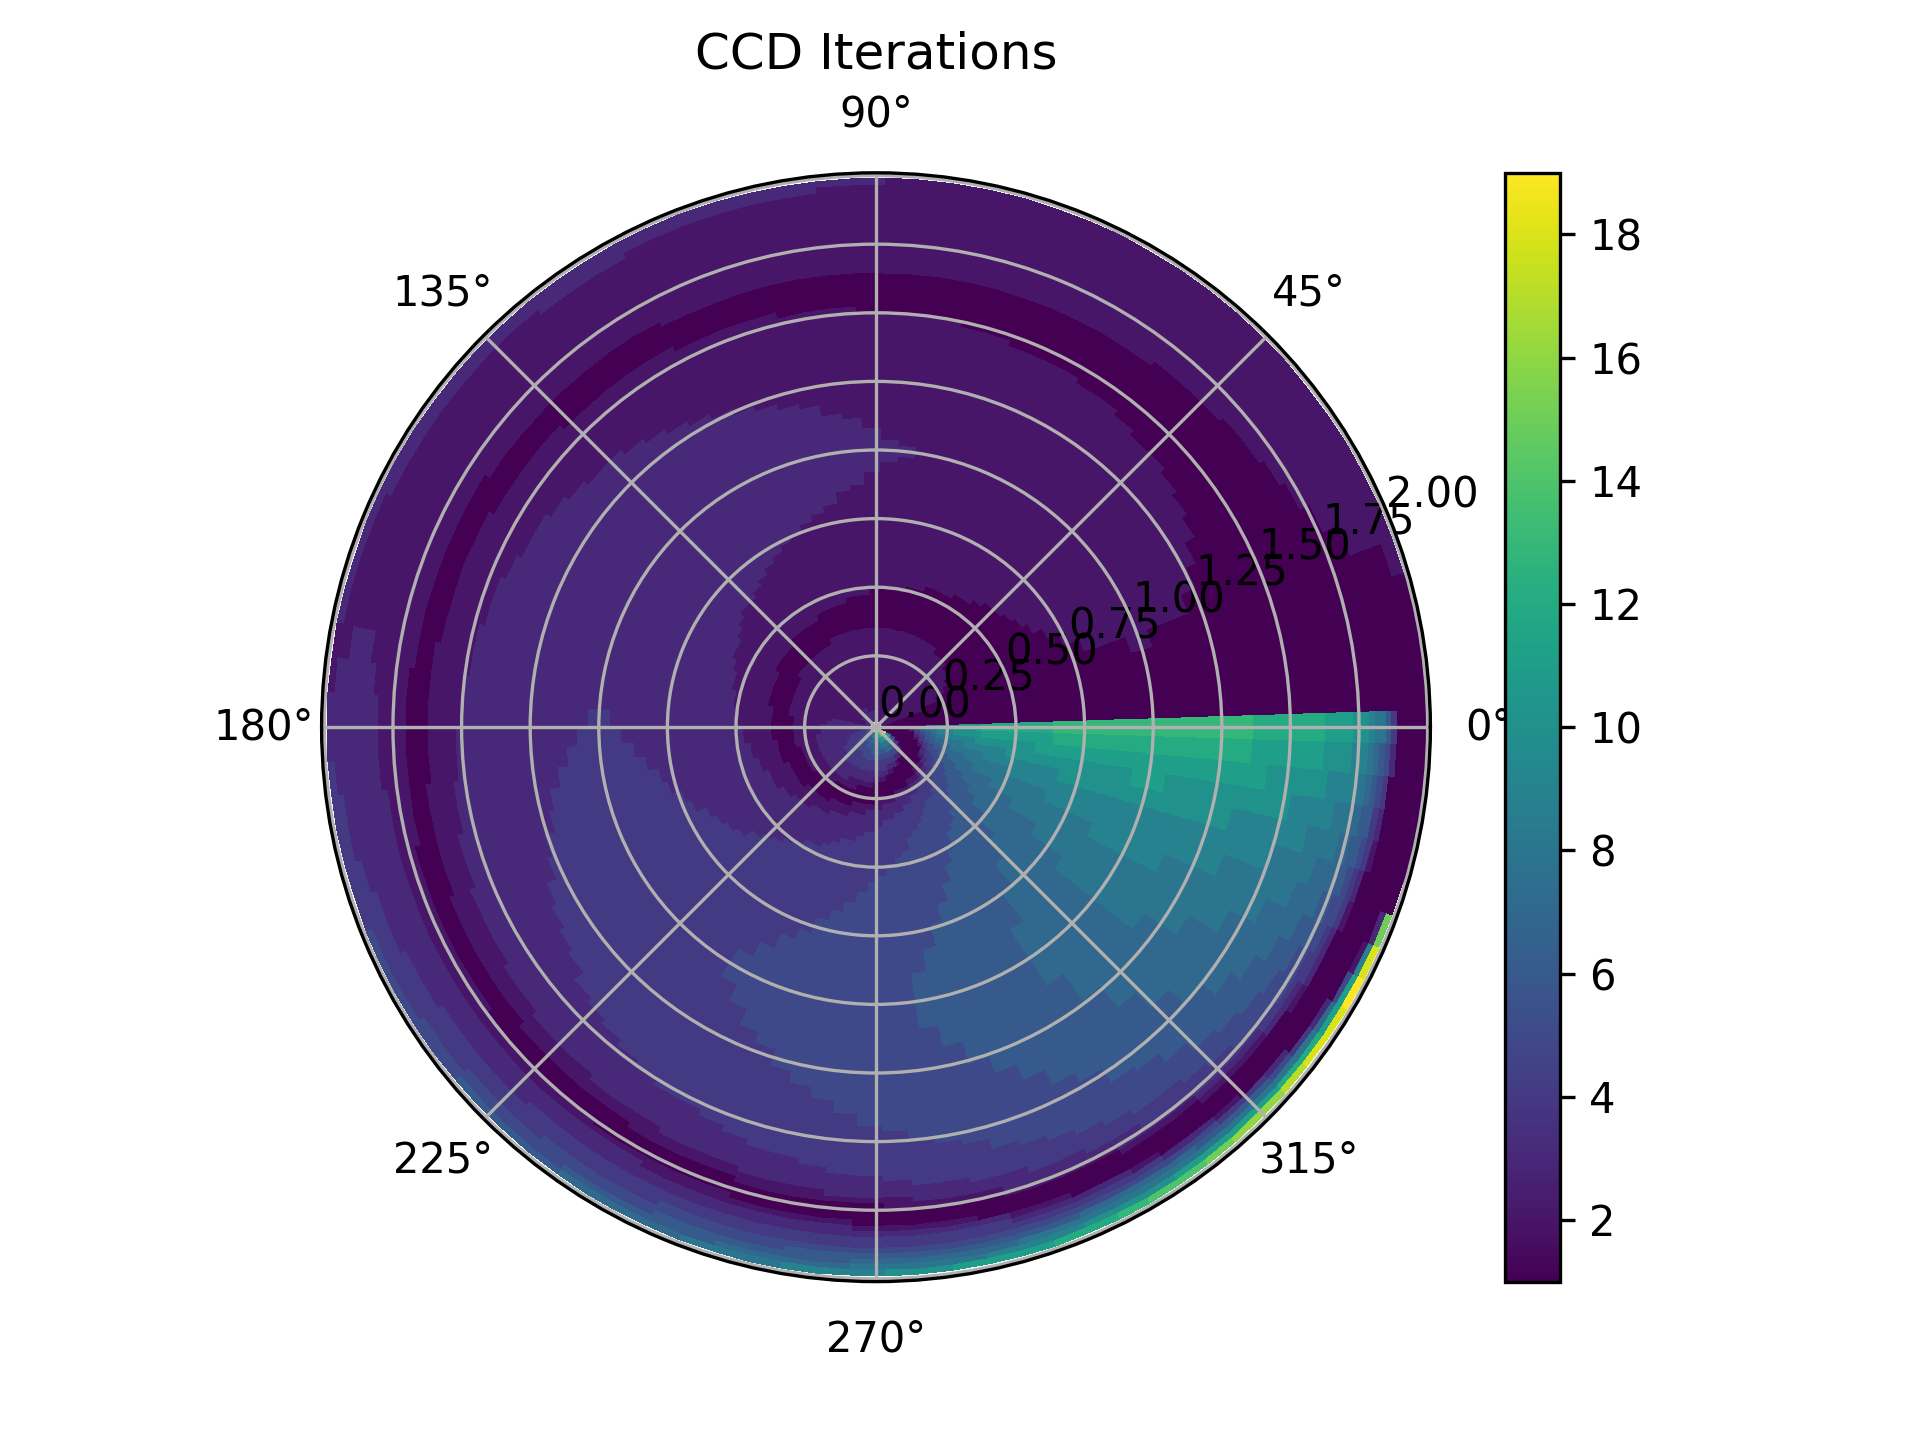
\includegraphics[width=0.31 \linewidth]{figures/background/CCD_2_iteration_heatmap.png}
            \label{fig:CCD_iteration/2}
            }
        \hfill
        \subfloat[$N = 5$]{
            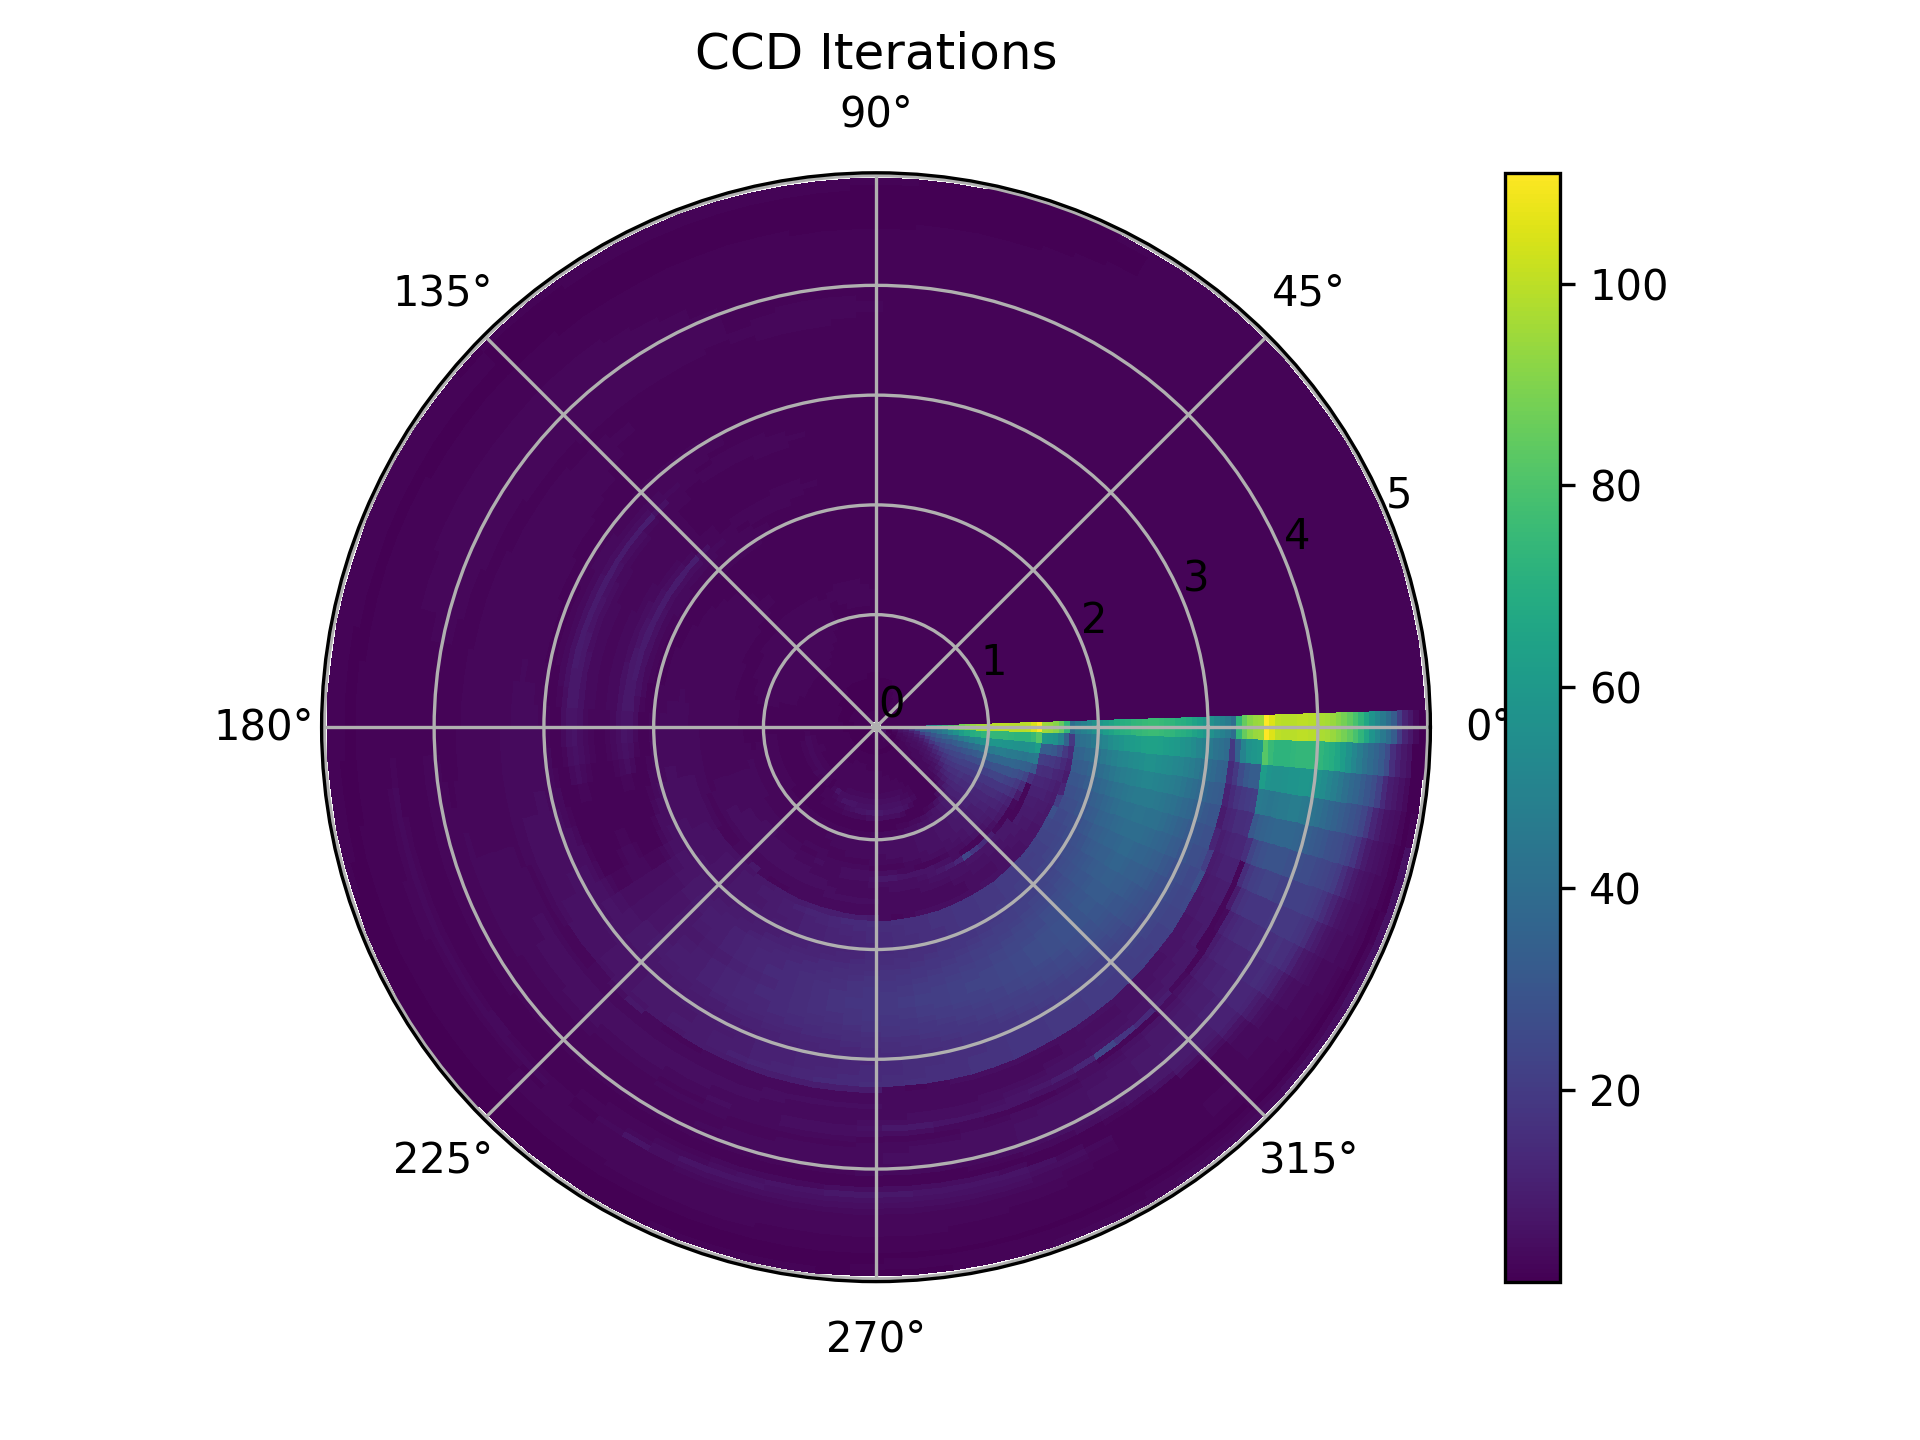
\includegraphics[width=0.31 \linewidth]{figures/background/CCD_5_iteration_heatmap.png}
            \label{fig:CCD_iteration/5}
            }
        \hfill
        \subfloat[$N = 10$]{
            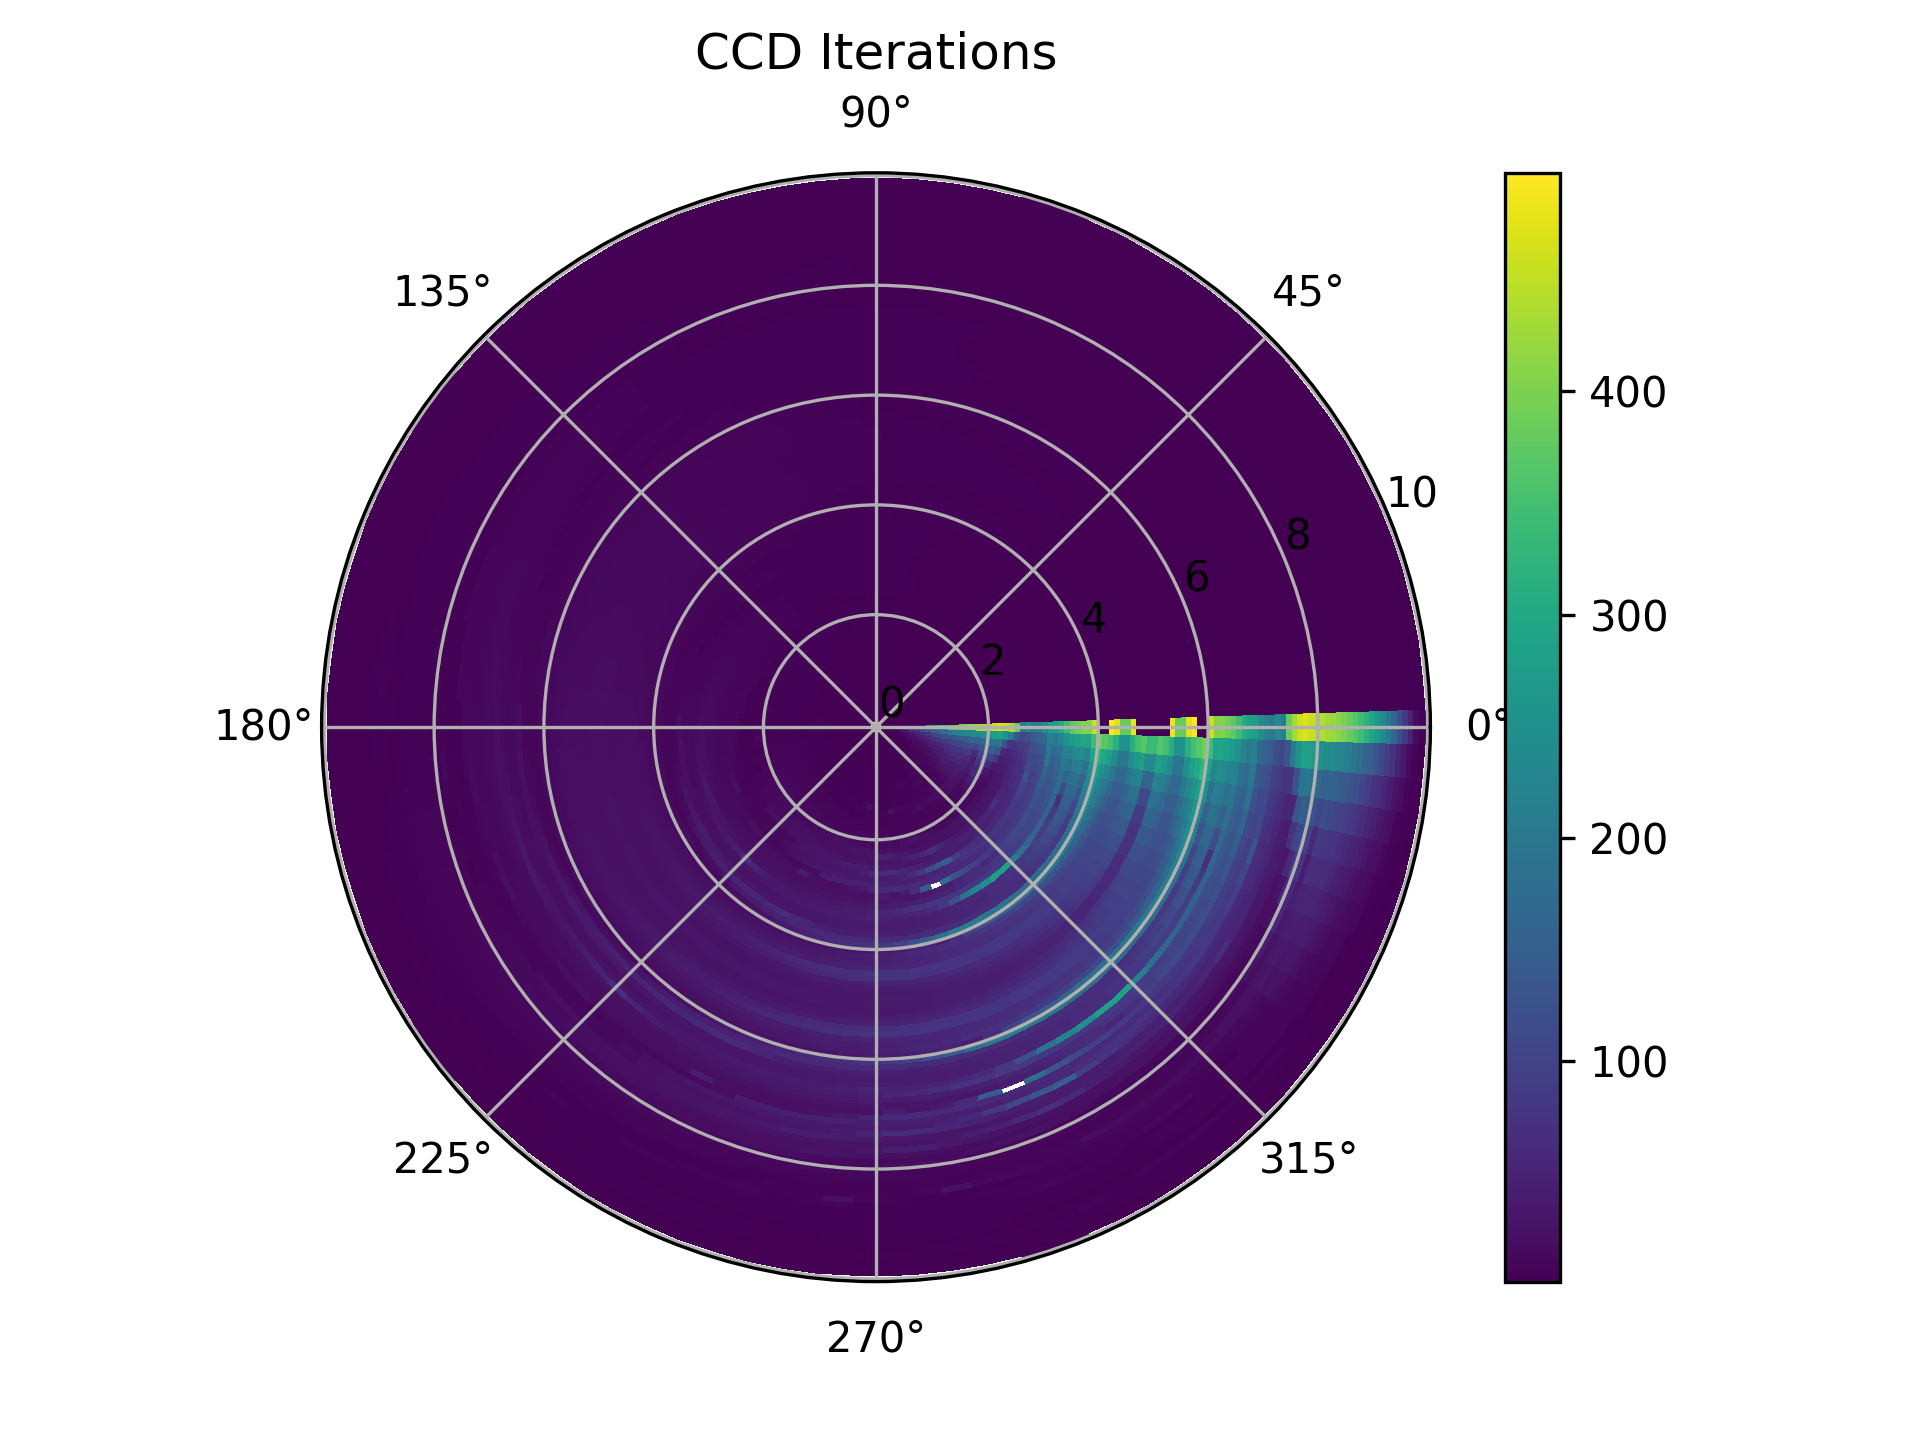
\includegraphics[width=0.31 \linewidth]{figures/background/CCD_10_iteration_heatmap.png}
            \label{fig:CCD_iteration/10}
            }
    \end{center}
    \caption[CCD iteration heatmap]{Heatmap of how many iterations CCD has needed to solve inverse kinematics starting from $[N, 0]$ targeting the middle of each polygon. The maximum budget is 20 times $N$ with a target precision of $0.1$.}
    \label{fig:CCD_iteration}
\end{figure}
\begin{figure}
    \begin{center}
        \subfloat[baseline. number of samples = 32062]{
            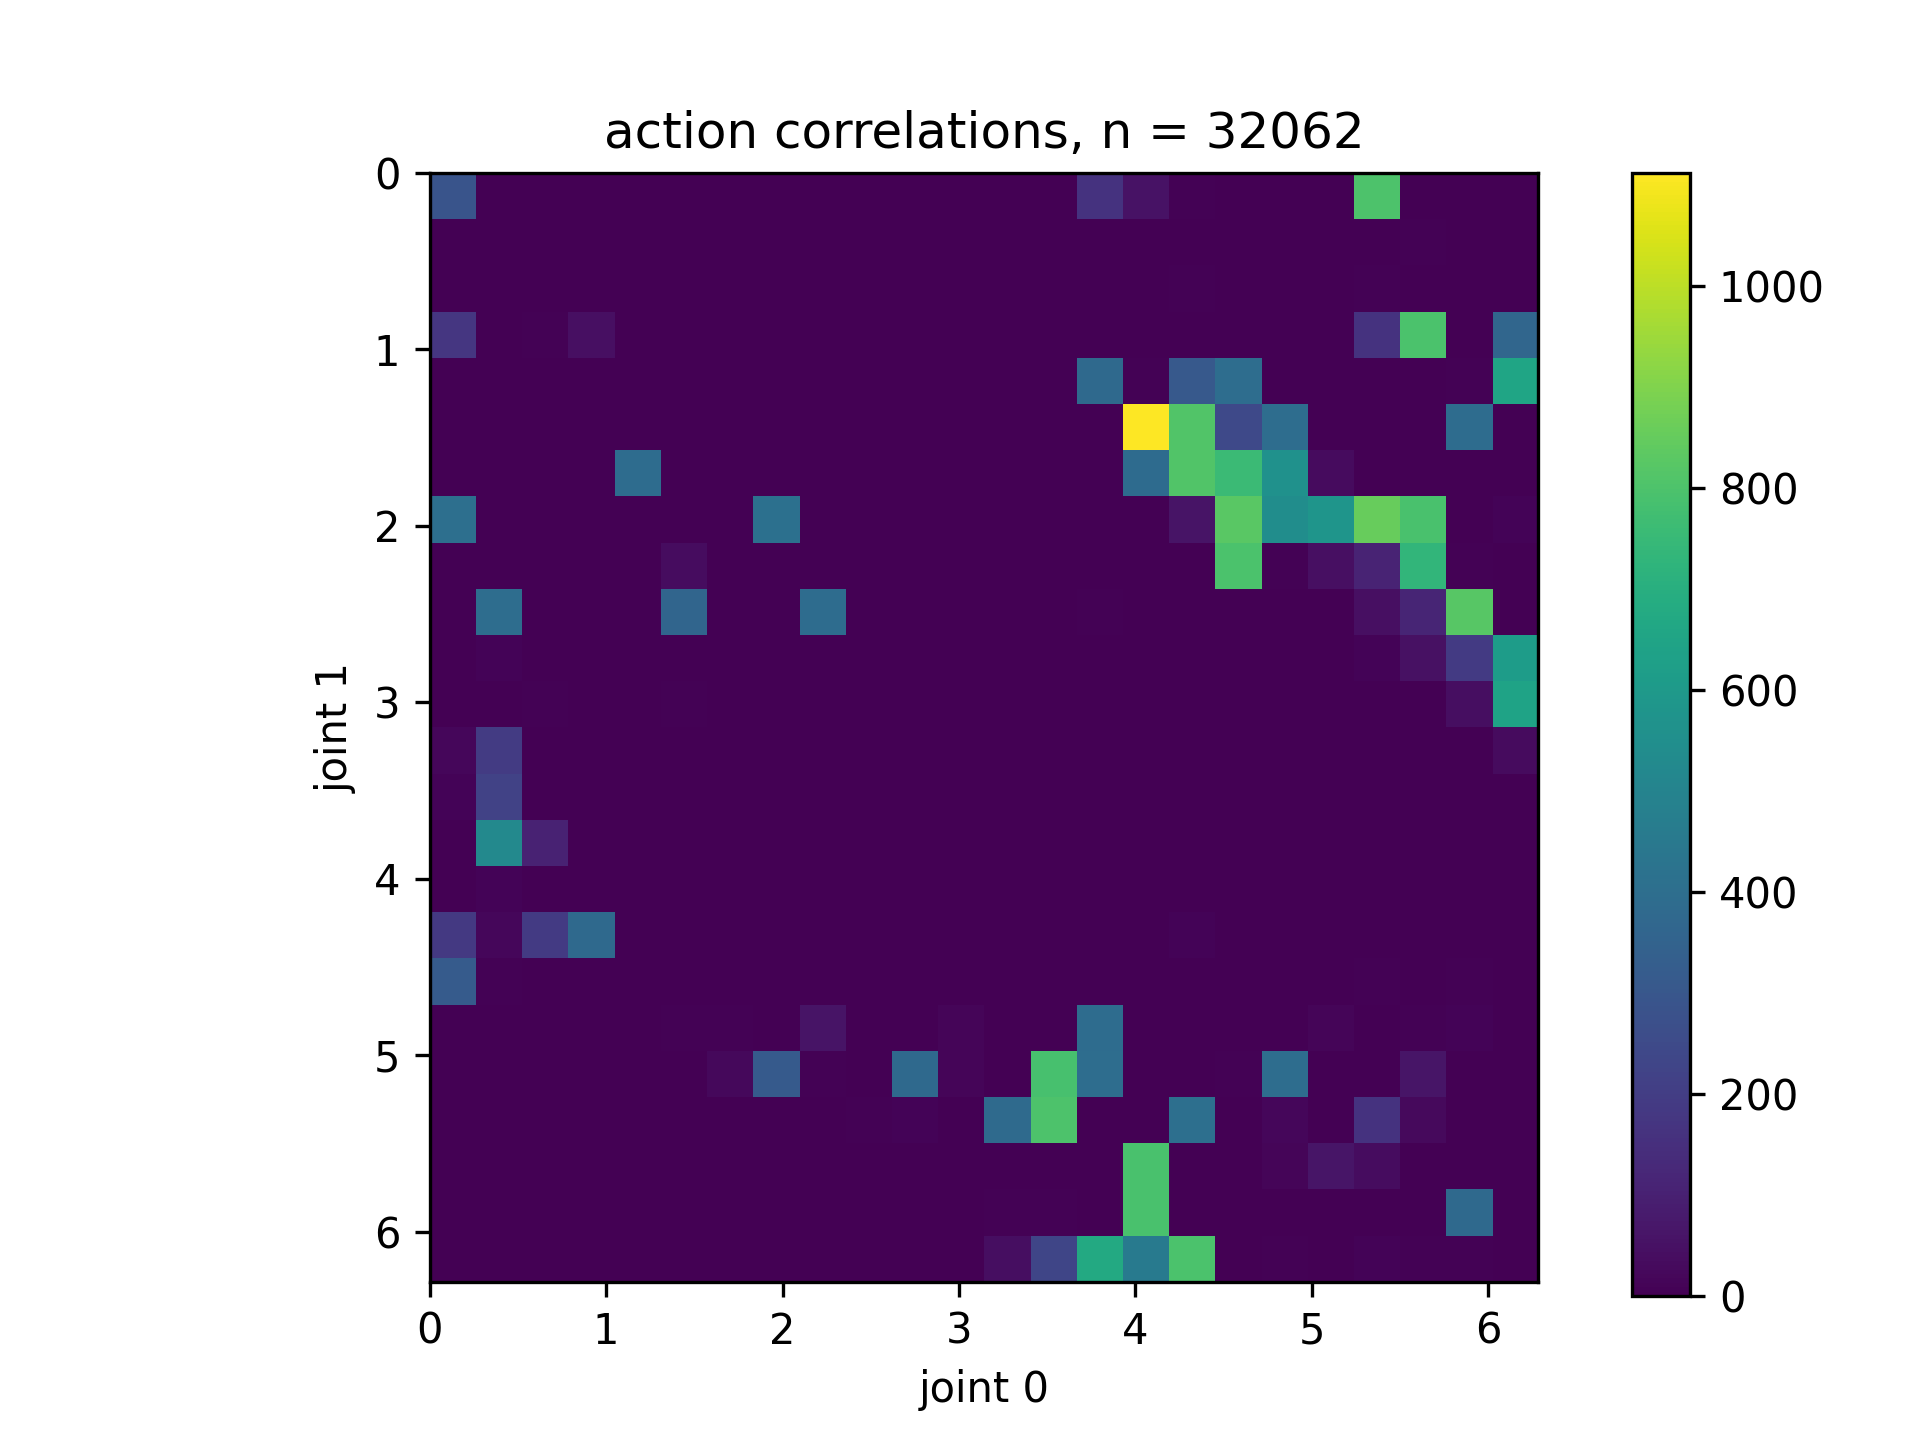
\includegraphics[width=0.23 \linewidth]{figures/experiments/action_correlations_baseline_2_1691621262_5000.png}
            \label{fig:SAC_action_correlation/baseline}
            }
        \hfill
        \subfloat[laten dimension is 2. number of samples = 39992]{
            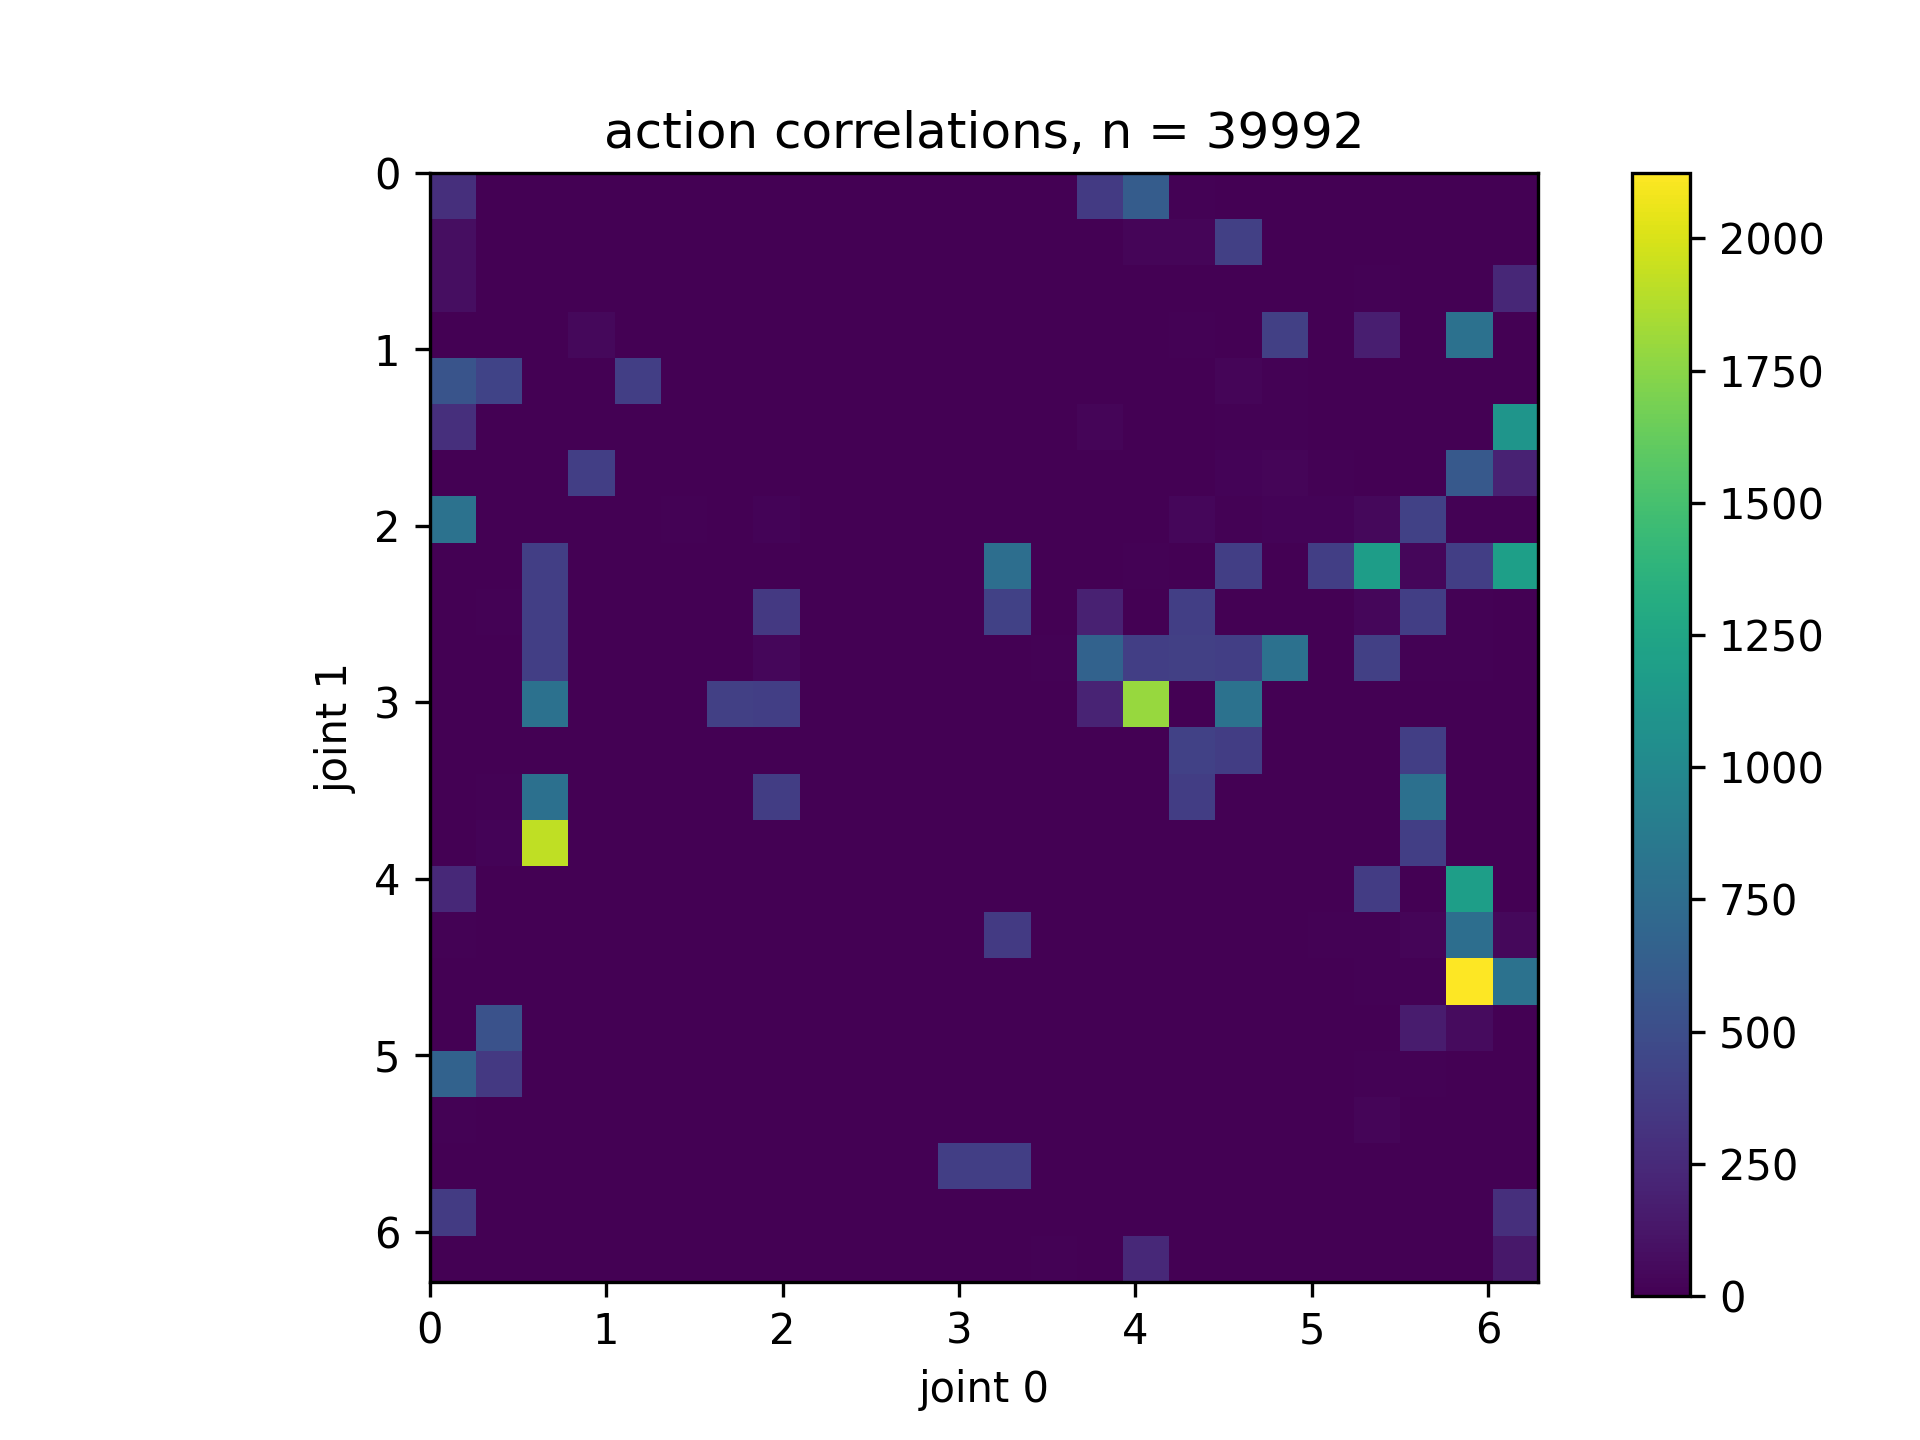
\includegraphics[width=0.23 \linewidth]{figures/experiments/action_correlations_latent_actor_2_2_1693146377_5000.png}
            \label{fig:SAC_action_correlation/latent_2}
            }
        \hfill
        \subfloat[laten dimension is 4. number of samples = 30810]{
            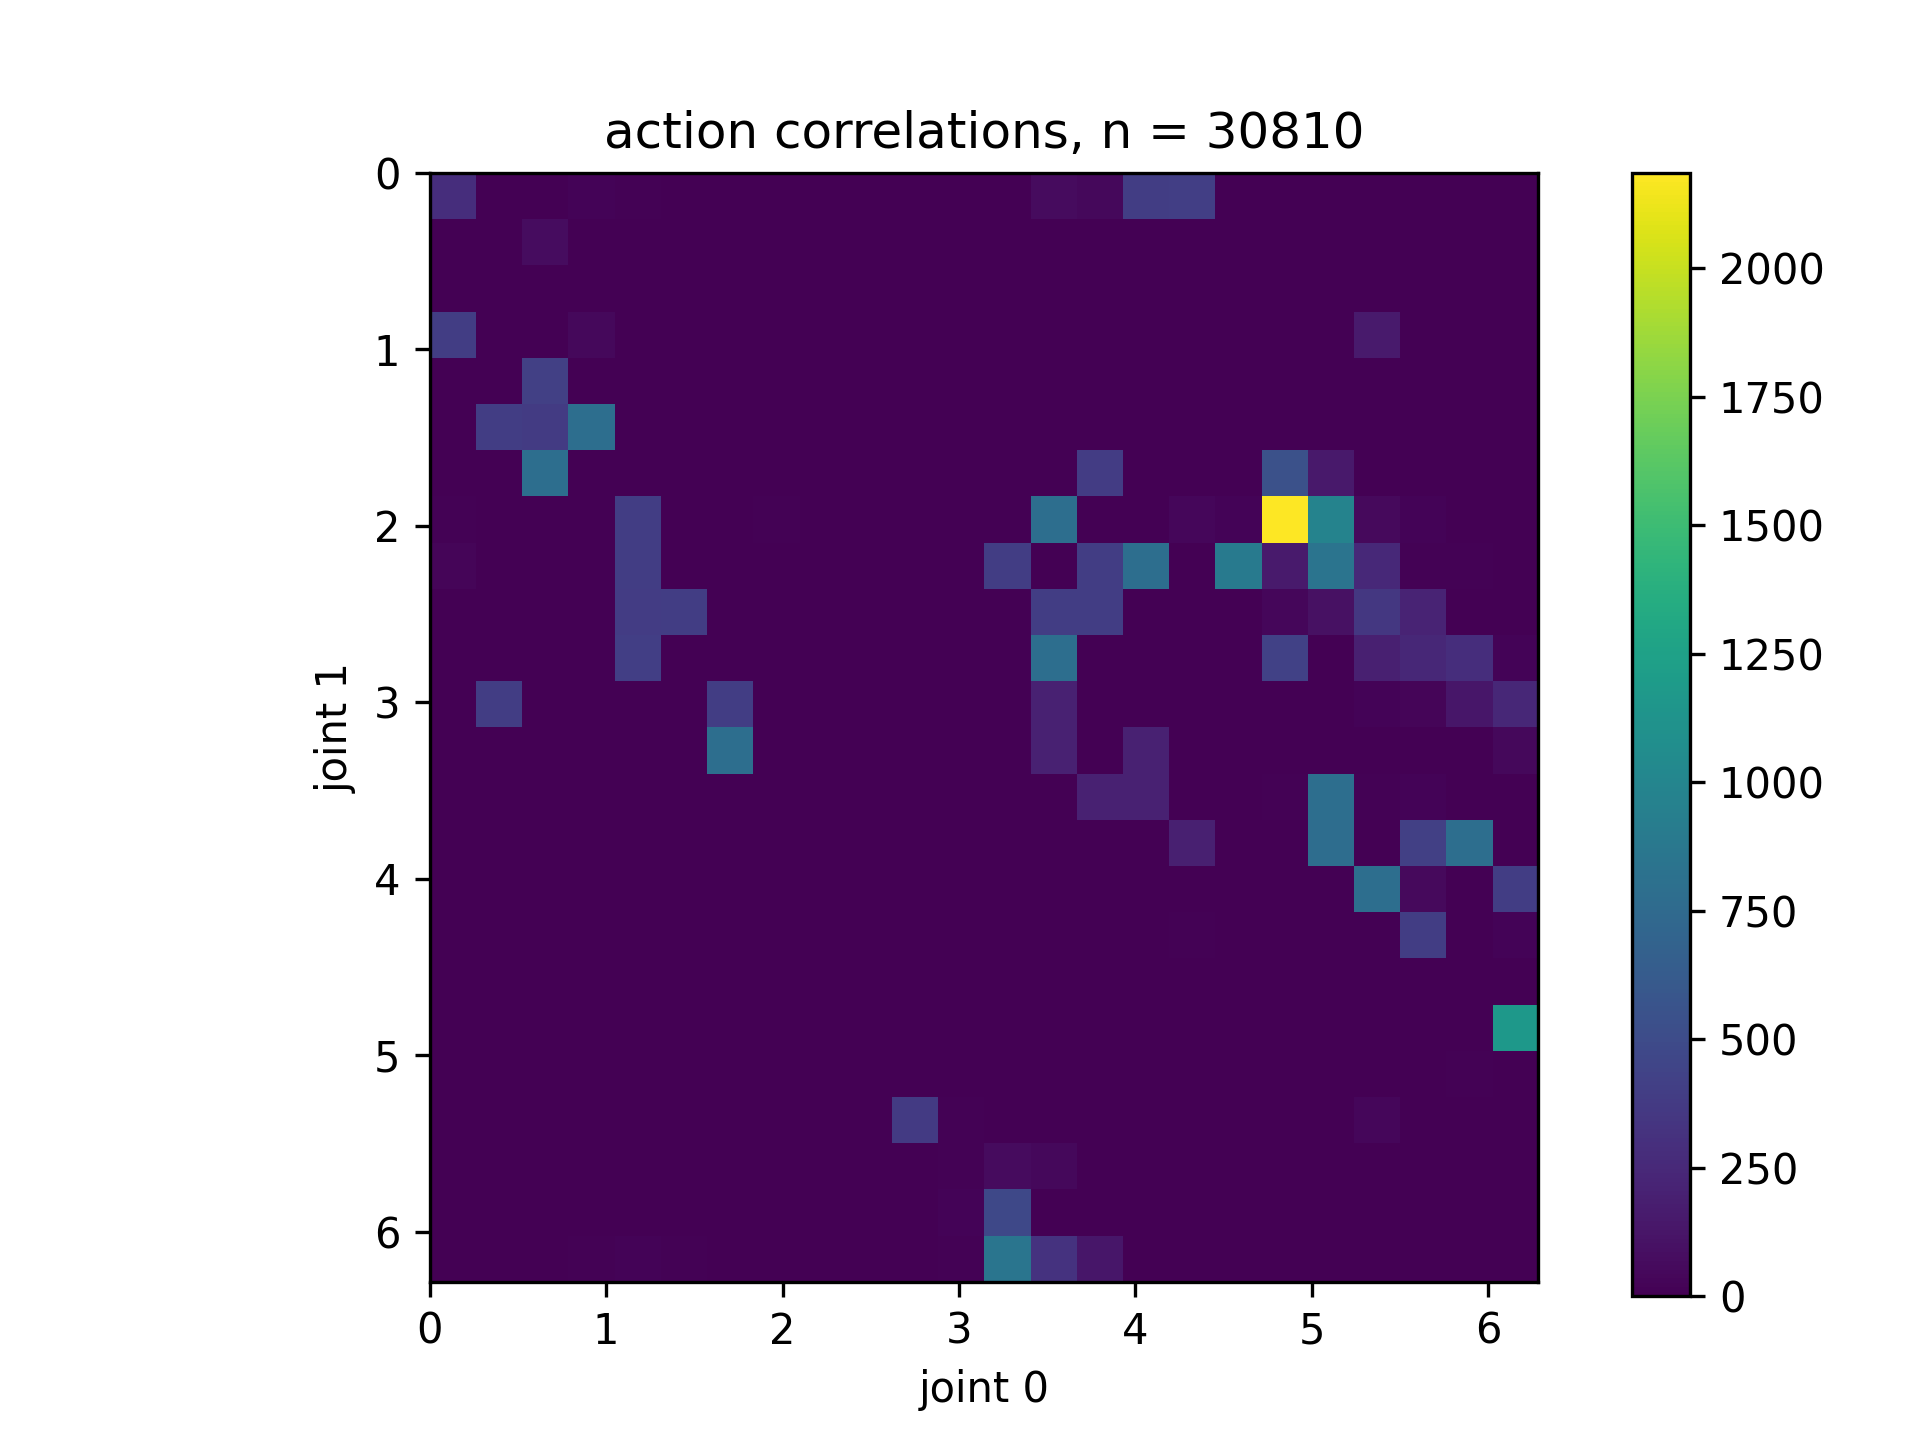
\includegraphics[width=0.23 \linewidth]{figures/experiments/action_correlations_latent_actor_4_2_1693063115_5000.png}
            \label{fig:SAC_action_correlation/latent_4}
            }
        \hfill
        \subfloat[laten dimension is 8. number of samples = 33247]{
            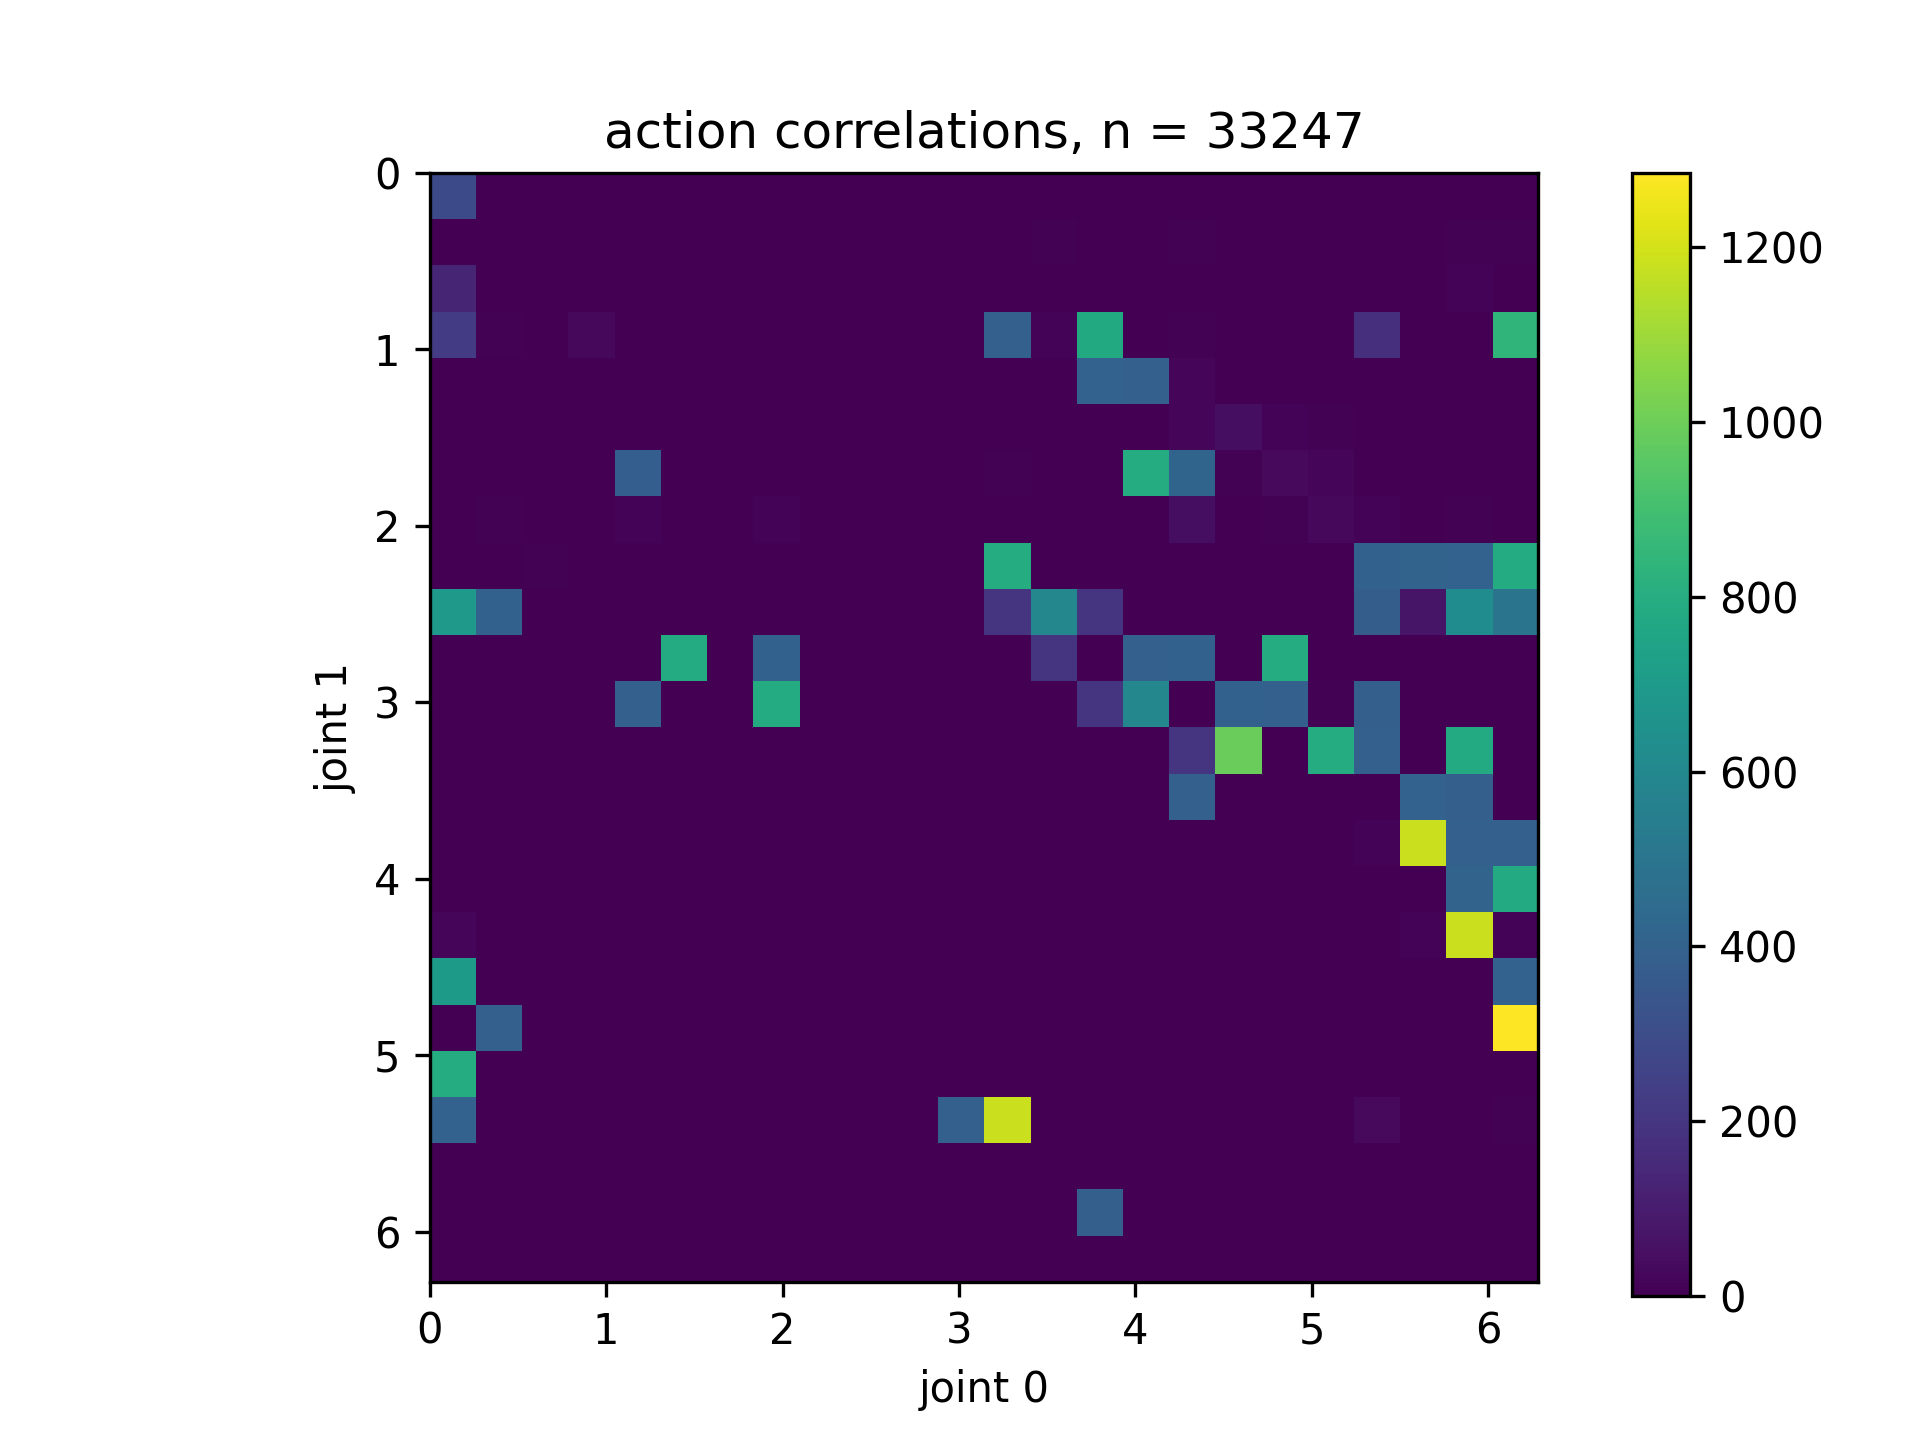
\includegraphics[width=0.23 \linewidth]{figures/experiments/action_correlations_latent_actor_8_2_1691615359_3000.png}
            \label{fig:SAC_action_correlation/latent_8}
            }
    \end{center}
    \caption[action correlation]{Plotted is the state angle correlation of two joints as a 2D histogram. The state angles are sampled from multiple episodes to uniformly sampled target positions. Each bucket can be translated to the number of angles in one 3D bucket $b$ with limits $b_{0, 0}, b_{0, 1}, b_{1, 0}, b_{1, 1}$. Mathematical speaking: $|b| = |\{q_t | q_t \in [0, 2\pi)^2 \land q_{0, t} \in [b_{0, 0}, b_{0, 1}] \land q_{1, t} \in [b_{1, 0}, b_{1, 1}]\}|$}
    \label{fig:SAC_action_correlation}
\end{figure}

\begin{table}
    \begin{center}
        \begin{tabular}{ l l | l l l l l}
        experiment series           & $N$                   & 2    & 5    & 10   & 15   & 20   \\
        \hline
        \hline
        \textit{baseline}           & $\mathfrak{S}$        & 0.73 & 0.83 & 0.57 & 0.42 & 0.30 \\
                                    & max eval $\bar{R_t}$  & 0.09 & 0.10 & 0.32 & 0.74 & 0.82 \\
        \hline
        \textit{latent 2}           & $\mathfrak{S}$        & 0.66 & 0.78 & 0.33 & 0.04 &      \\
                                    & max eval $\bar{R_t}$  & 0.11 & 0.15 & 0.83 & 3.62 &      \\
        \hline
        \textit{latent 4}           & $\mathfrak{S}$        & 0.76 & 0.84 & 0.54 & 0.04 &      \\
                                    & max eval $\bar{R_t}$  & 0.09 & 0.09 & 0.50 & 3.89 &      \\
        \hline
        \textit{latent 8}           & $\mathfrak{S}$        & 0.72 & 0.88 & 0.22 & 0.06 &      \\
                                    & max eval $\bar{R_t}$  & 0.09 & 0.08 & 2.97 & 4.22 &      \\
        \hline
        \textit{latent imitation}   & $\mathfrak{S}$        & 0.85 & 0.85 & 0.45 & 0.11 &      \\
                                    & max eval $\bar{R_t}$  & 0.08 & 0.10 & 0.44 & 2.01 &      \\
        \hline
        \textit{super distance}     & $\mathfrak{S}$        & 0.62 & 0.60 & 0.53 &      &      \\
                                    & max eval $\bar{R_t}$  & 0.11 & 0.20 & 0.64 &      &      \\
        \hline
        \textit{super imitation}    & $\mathfrak{S}$        & 0.19 & 0.25 & 0.21 &      &      \\
                                    & max eval $\bar{R_t}$  & 0.37 & 0.34 & 0.71 &      &      \\
    \end{tabular}
    \end{center}
    \caption[SAC Solved ratio]{Solved ratio $\mathfrak{S}$ and closest distance to target during one episode as known as the maximum reward during one episode for one target position, for all SAC experiments starting at $[N, 0]$ and targeting the same targets as in \figref{fig:SAC_baseline_min_distances} with a maximal budget of 400 steps. Those are examples from individual experiments all from epoch 3000. For more details on which experiments please have a look at the figures directory. The suffix of each png describes where to find the experiment. For a closer inspection of how the individual models perform over the evaluation please refer to \chapref{chap:appendix}}
    \label{tab:SAC_solved_ratio}
\end{table}

A comparison between CCD and baseline SAC revealed several intriguing distinctions:

\begin{itemize}
    \item \textbf{Target Dependence}: Upon closer examination of CCD, it became evident that its performance in a single run was significantly influenced by the initial configuration and the specific target location. This was well-illustrated in  \figref{fig:CCD_iteration}, which depicted CCD's performance in terms of the number of iterations required to reach the desired target position. Interestingly, when we analyzed the steps needed to reach the target position using SAC, a noteworthy trend emerged. As the number of joints increased, we found that SAC more frequently reached the maximum iteration limit rather than successfully reaching the target as illustrated in \chapref{chap:appendix} and \tabref{tab:SAC_solved_ratio}. One potential explanation, alluded to in \figref{fig:SAC_baseline_inference_trajectory}, was that the agent's behavior sometimes declined as it neared the target. After coming tantalizingly close, the end-effector would rapidly retreat towards the arms origin, failing to get as close to the desired target as before. This observation was backed up by \figref{fig:SAC_baseline_min_distance_step}, which showed that the minimum distance to the target was typically achieved in around 50 steps or fewer during an episode. It's worth noting that this difficulty in reaching the target could be attributed to SAC's fixed threshold for ending an episode, which required a $0.1$ Euclidean distance between the end-effector and the target by definition. As the number of joints increased, the area within which the end-effector's position could end an episode diminished quadratically, making it progressively harder to reach the target with more joints. However, this argument was counterbalanced by the fact that the robot arm could execute more precise movements or potentially decompose the problem into smaller parts. For instance, joint $1$ to $N-2$ could be utilized to roughly position the end-effector near the target, while joint $N-1$ to $N$ could perform the precise adjustments. This raises a crucial question: why did the agent consistently fail, often by a substantial margin, after coming so close to the target? One plausible explanation is that the agent frequently encountered scenarios where it almost reached the target but had no opportunity to learn from these experiences. On the contrary, the extended episode length and increasing failure rate while increasing $N$, as seen in  \tabref{tab:SAC_solved_ratio}, should work against this trend.
    \item \textbf{Solutions}: A deeper exploration of how SAC and CCD tackled inverse kinematics problems unveiled a strong contrast in the distribution of state angles. Comparing \figref{fig:dataset_action_correlation}, which depicted the state angle distribution required to reach the target in the dataset, with \figref{fig:SAC_action_correlation/baseline}, which illustrated the distribution resulting from baseline SAC, highlighted this discrepancy. While the former exhibited a rhombus-shaped distribution, the latter showcased a more scattered pattern.
\end{itemize}

It is important to recognize that this qualitative comparison between CCD and SAC is inherently limited. CCD enjoys unrestricted access to the entire action space, whereas SAC's action range is constrained due to action normalization. It's also noteworthy that scaling the hyperbolic tangent output to a range of $2\pi$ or higher, while a potential solution, is not without its challenges. Doing so could lead to SAC finding multiple actions that yield the same action outcome or potentially complicate the calculation of log probabilities for the policy.

At this juncture, we can draw connections between our baseline experiments and the concepts presented in the Motor Synergy paper \cite{Motor_Synergy_Learning}. An interesting proposition arises when we closely examine the inverse kinematics problem as defined in the environment description. One conceivable strategy involves dividing the robot arm into two sections, each comprising $N/2$ segments, and constraining the relative angles within each segment. These two segments would effectively resemble a robot arm with just two extended joints. As previously demonstrated, environments with two joints are quite tractable. Yet, why doesn't the policy opt for such a strategy? Several arguments come to the fore. It's plausible that this strategy results in a longer trajectory to reach the target, which could affect the accumulated reward. Additionally, the choice could be influenced by the exploration strategy, as increasing entropy to encourage exploration does not seem effective due to the collapsing distribution, as seen in \figref{fig:Uniform_dataset}.

The decrease in SAC's performance, as evidenced in \figref{fig:SAC_baseline}, can also be attributed to the linear growth in the complexity of the observation space, given that $S$ is a subset of $\mathbb{R}^{4+N}$. To address this escalating complexity, researchers might consider increasing the number of hidden layers or neurons per layer while delving into neural architecture search. An alternative approach for investigating this theory could involve the application of Neural-Evolution-of-Augmented-Topologies (NEAT). This algorithm seeks to identify the smallest neural architecture capable of solving a given task. Given the context provided, it's reasonable to assume that the discovered neural architecture becomes increasingly complex as $N$ increases.




\begin{figure}
    \begin{center}
        \subfloat[$N = 2$]{
            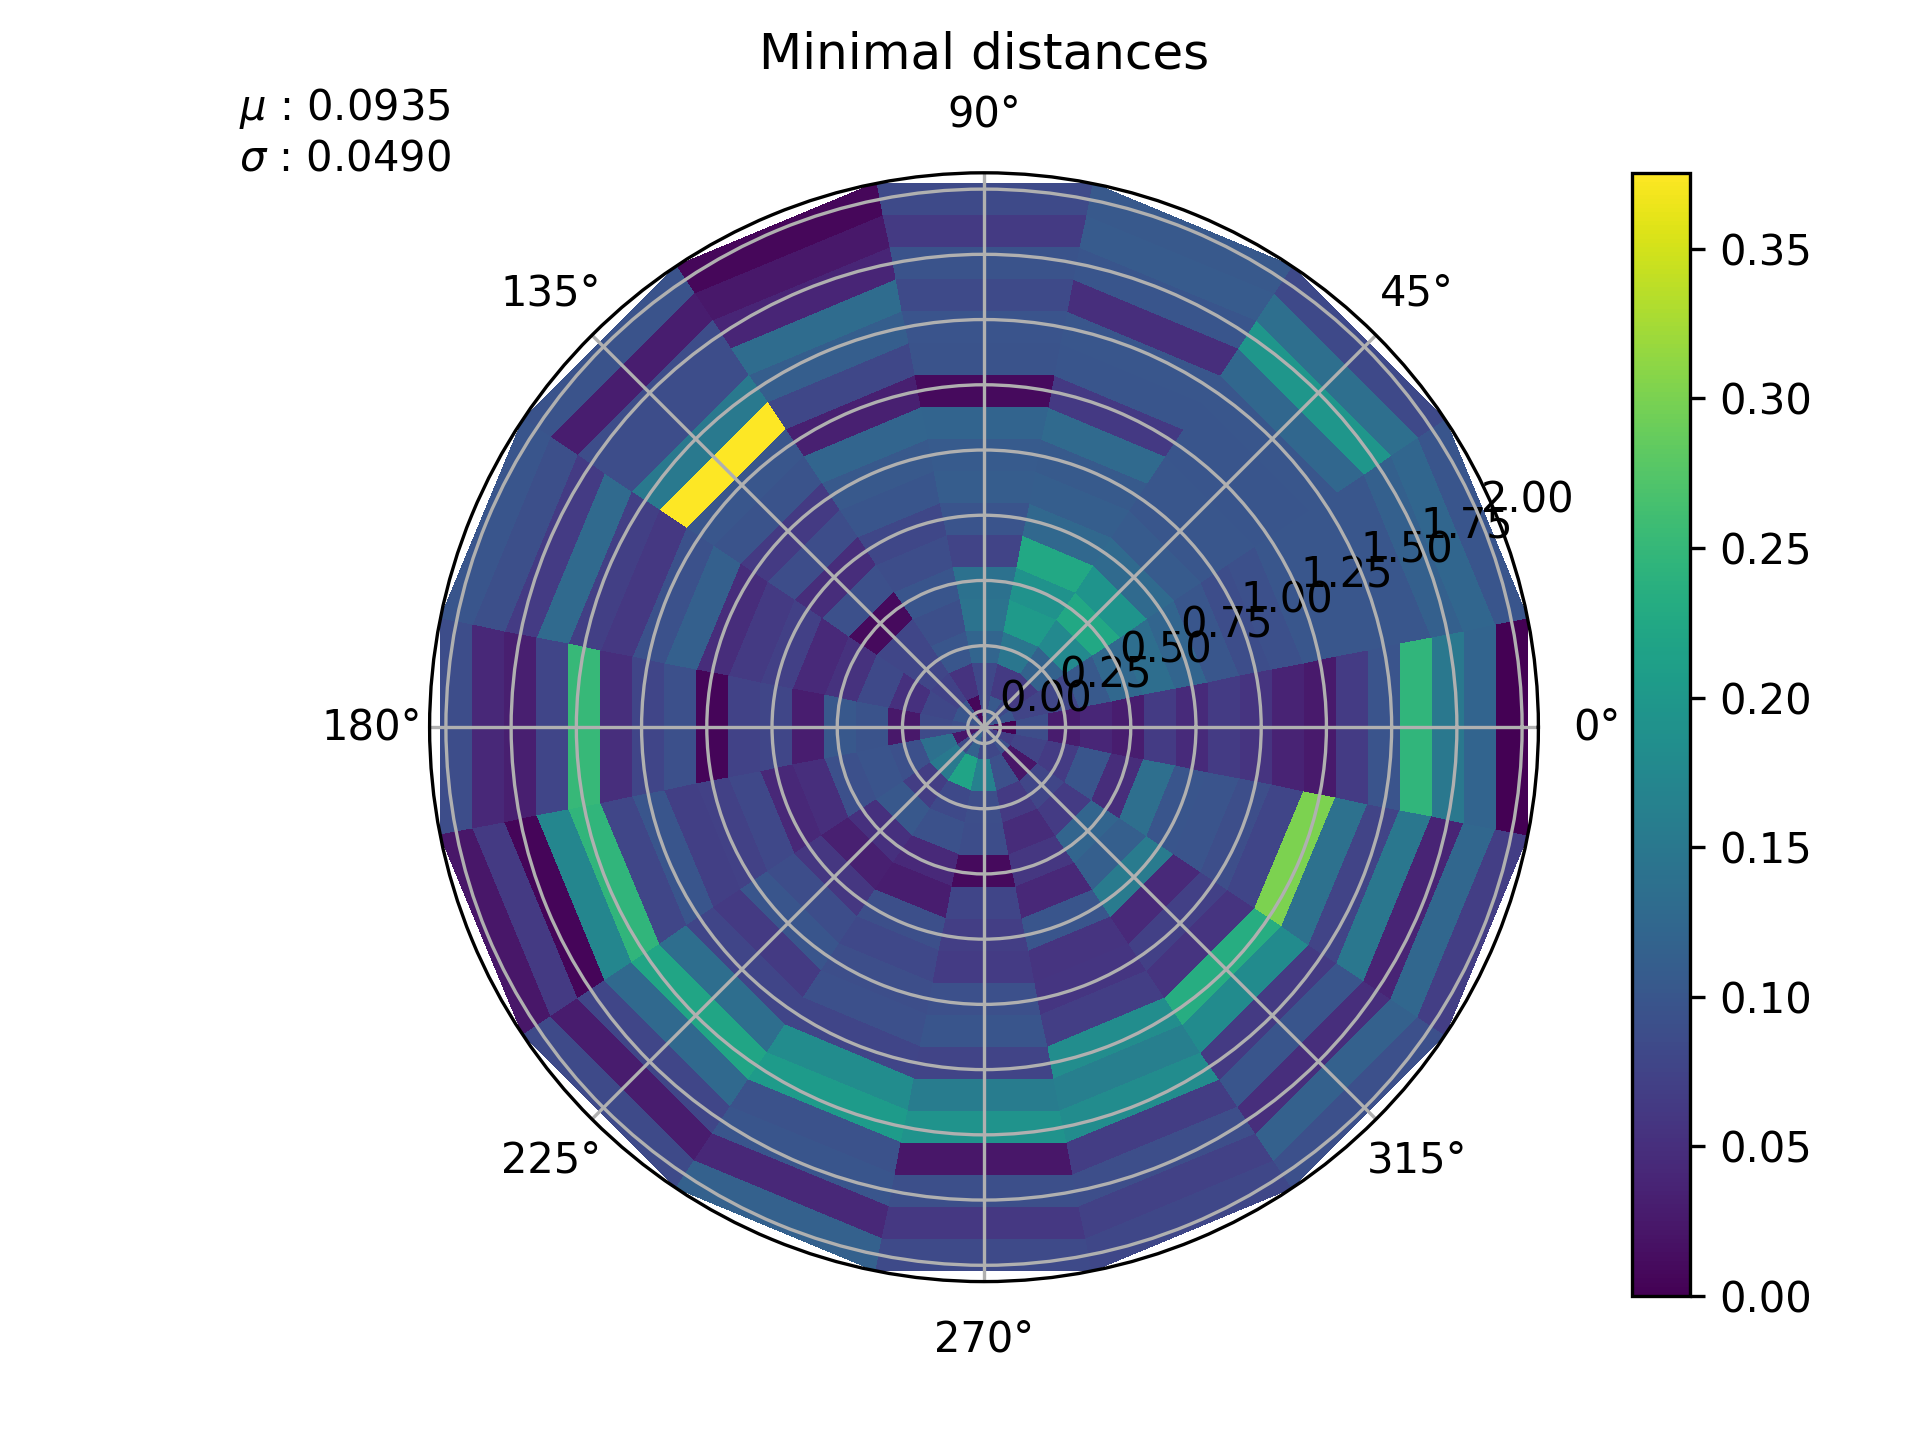
\includegraphics[width=0.31 \linewidth]{figures/experiments/Minimal_distances_baseline_2_1691621262_5000.png}
            \label{fig:SAC_baseline_min_distances/2}
            }
        \hfill
        \subfloat[$N = 5$]{
            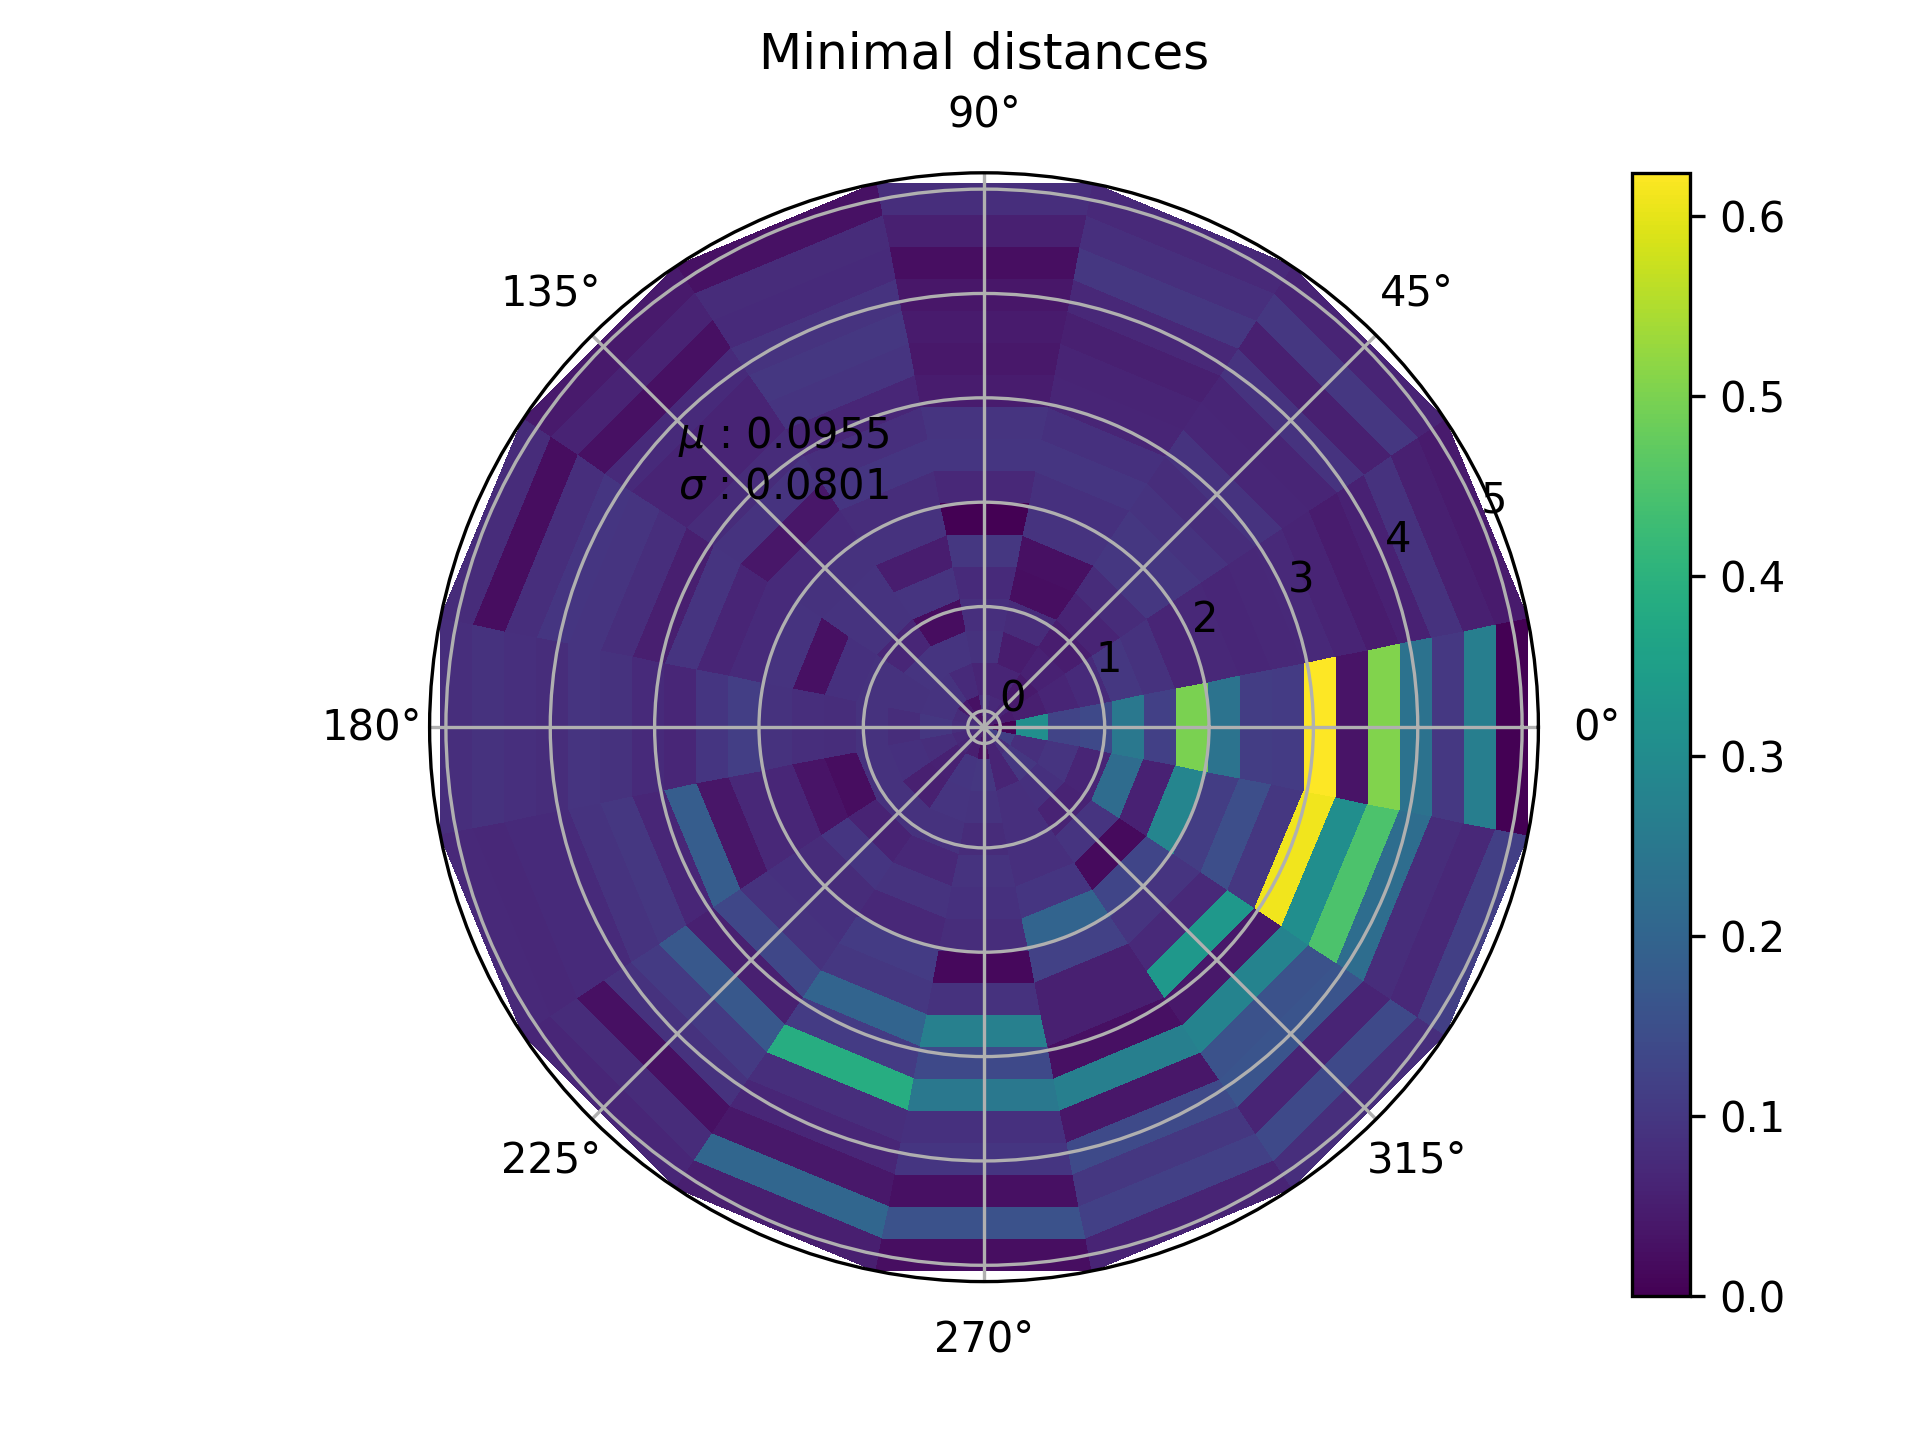
\includegraphics[width=0.31 \linewidth]{figures/experiments/Minimal_distances_baseline_5_1691621331_5000.png}
            \label{fig:SAC_baseline_min_distances/5}
            }
        \hfill
        \subfloat[$N = 10$]{
            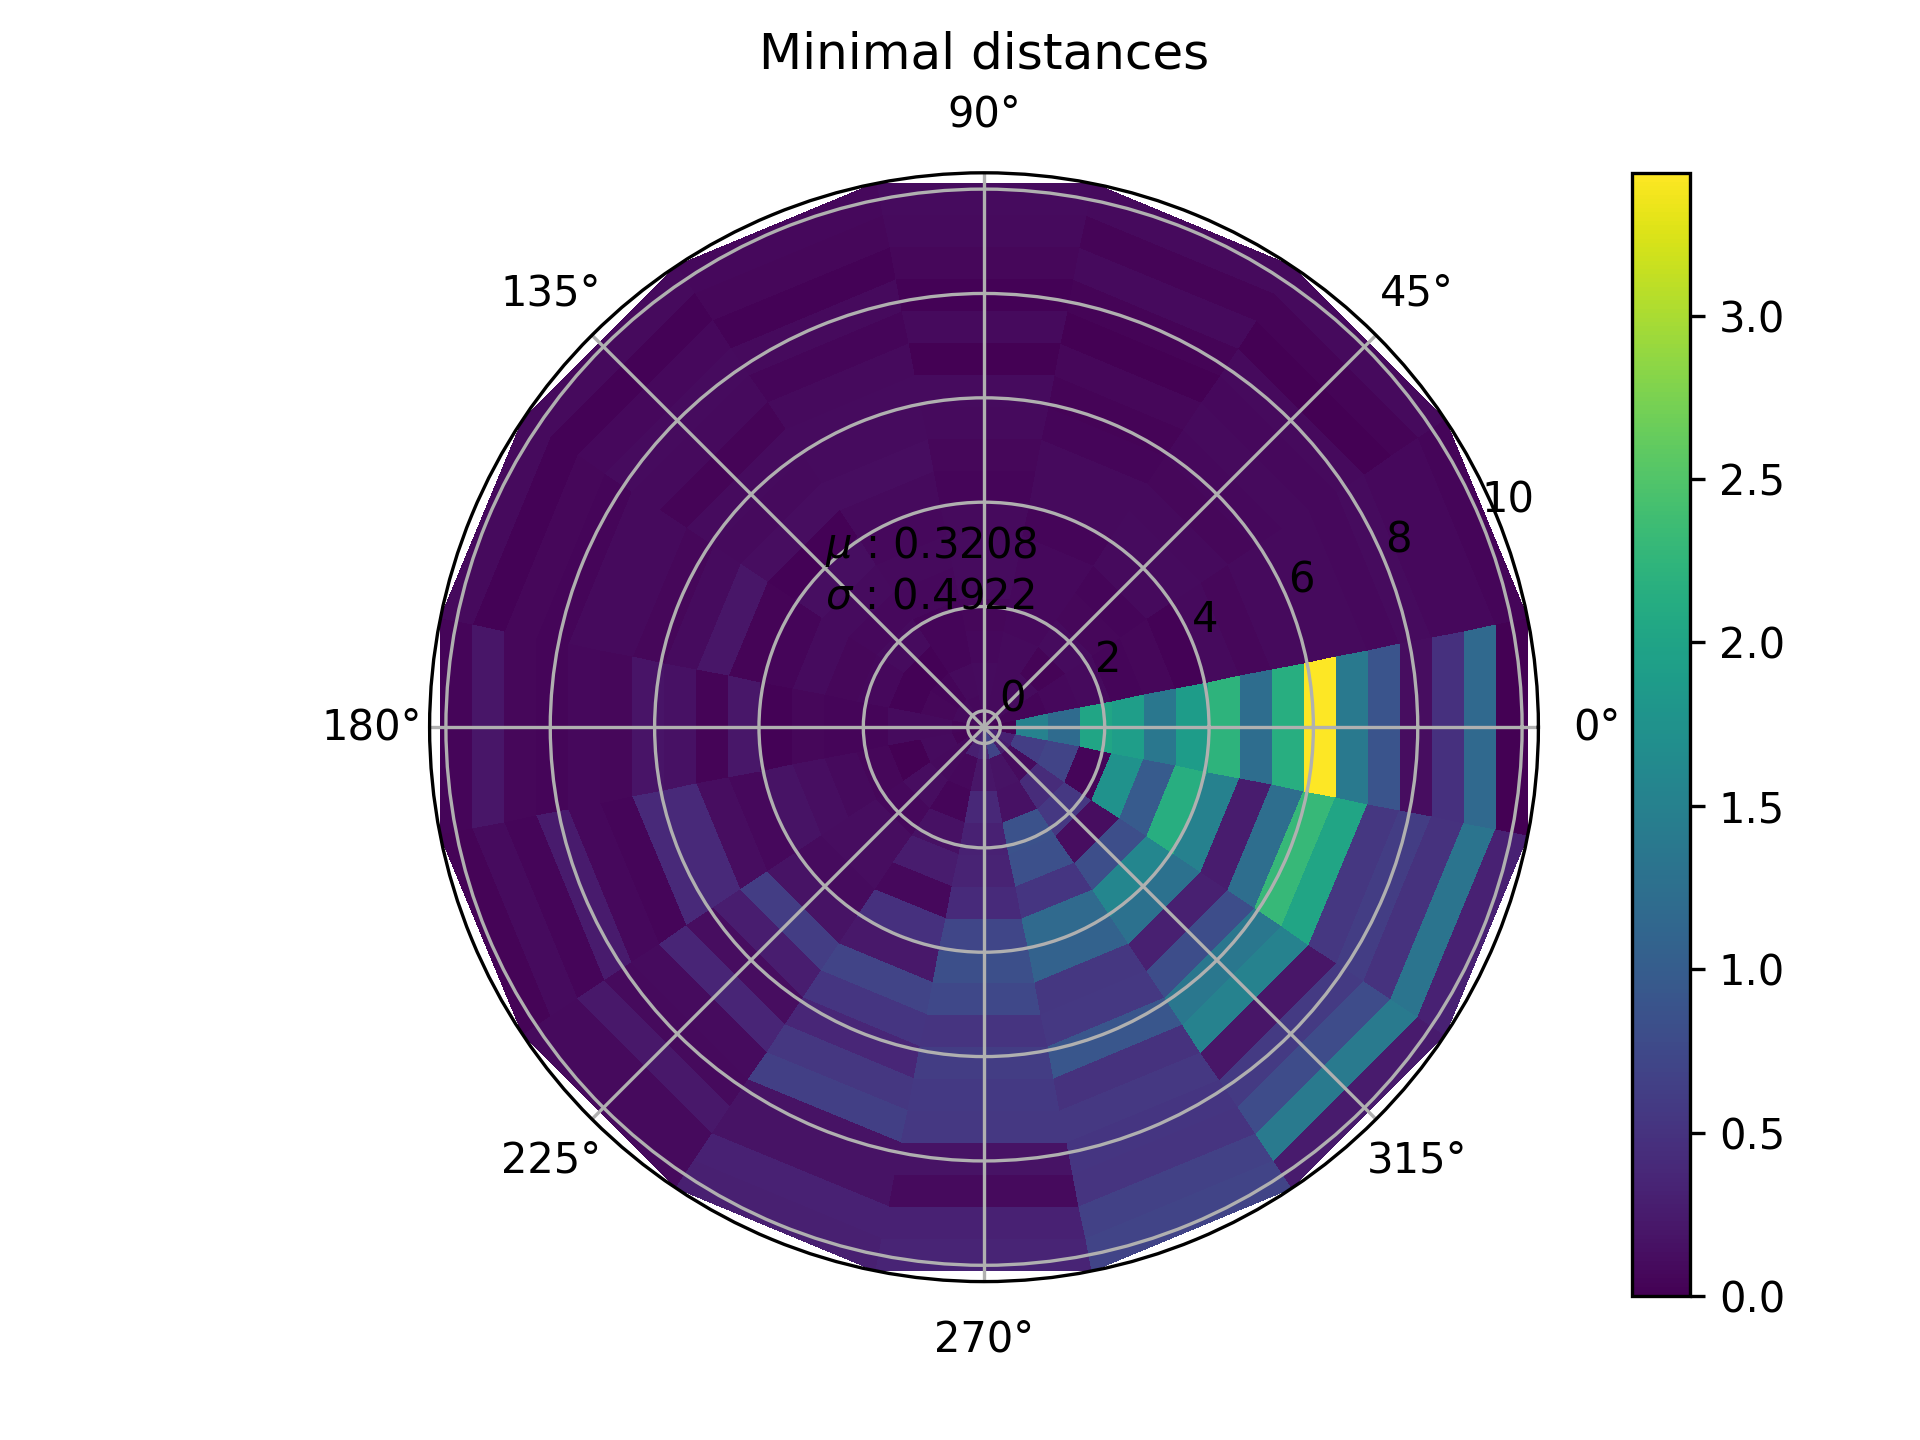
\includegraphics[width=0.31 \linewidth]{figures/experiments/Minimal_distances_baseline_10_1691618968_5000.png}
            \label{fig:SAC_baseline_min_distances/10}
            }
    \end{center}
    \caption[SAC min distance heatmap]{Minimal distance to a target during inference starting from $[N , 0]$ and targeting the middle of each polygon.}
    \label{fig:SAC_baseline_min_distances}
\end{figure}


\begin{figure}
    \begin{center}
        \subfloat[$N = 2$]{
            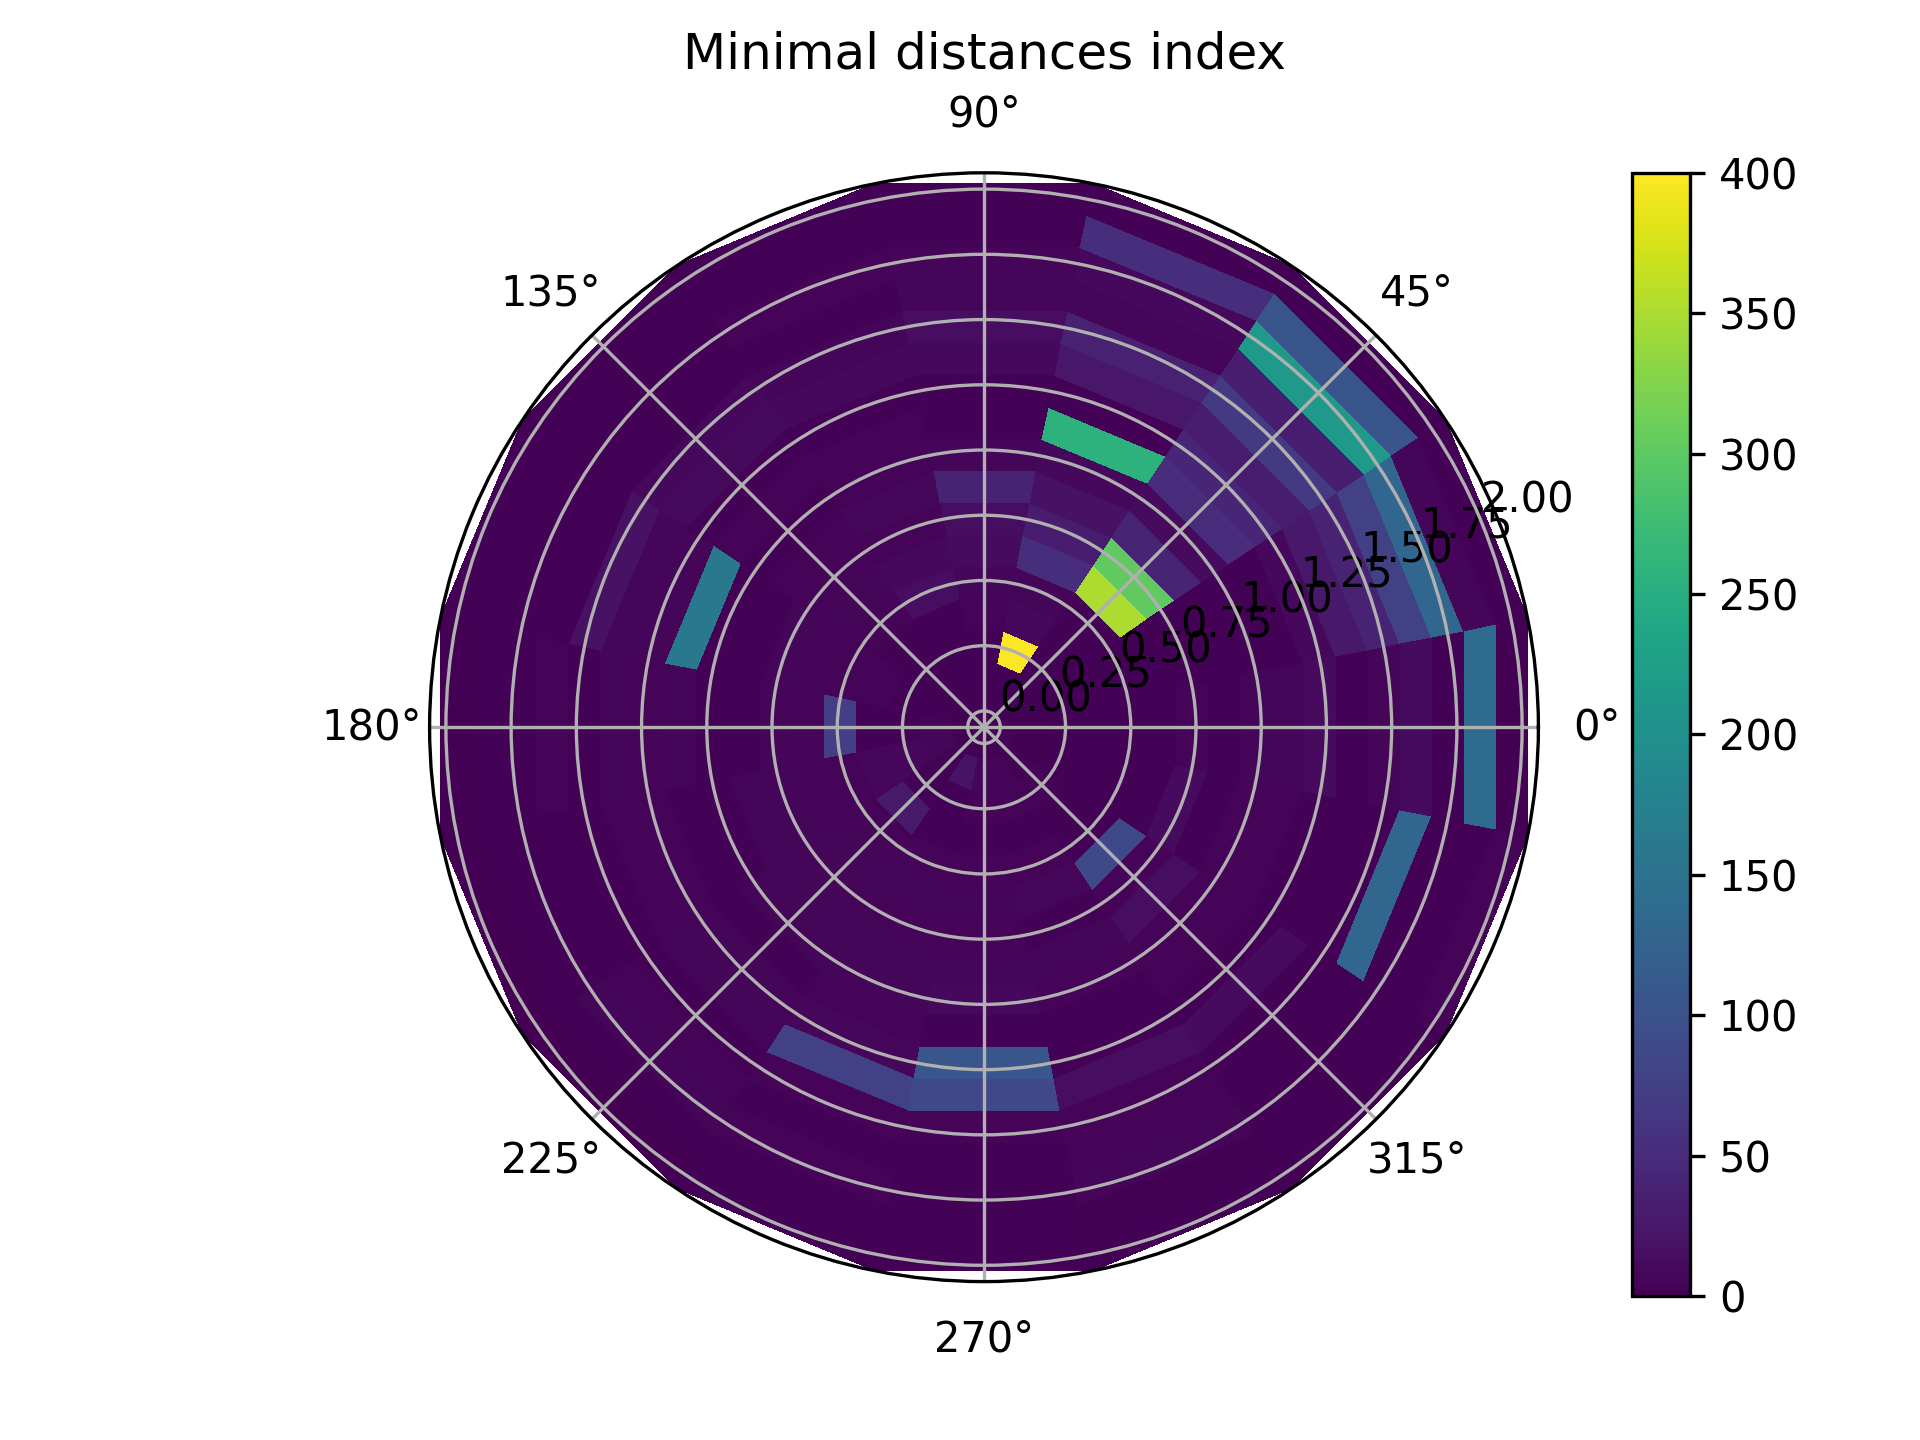
\includegraphics[width=0.31 \linewidth]{figures/experiments/Minimal_distances_index_baseline_2_1691621262_5000.png}
            \label{fig:SAC_baseline_min_distance_step/2}
            }
        \hfill
        \subfloat[$N = 5$]{
            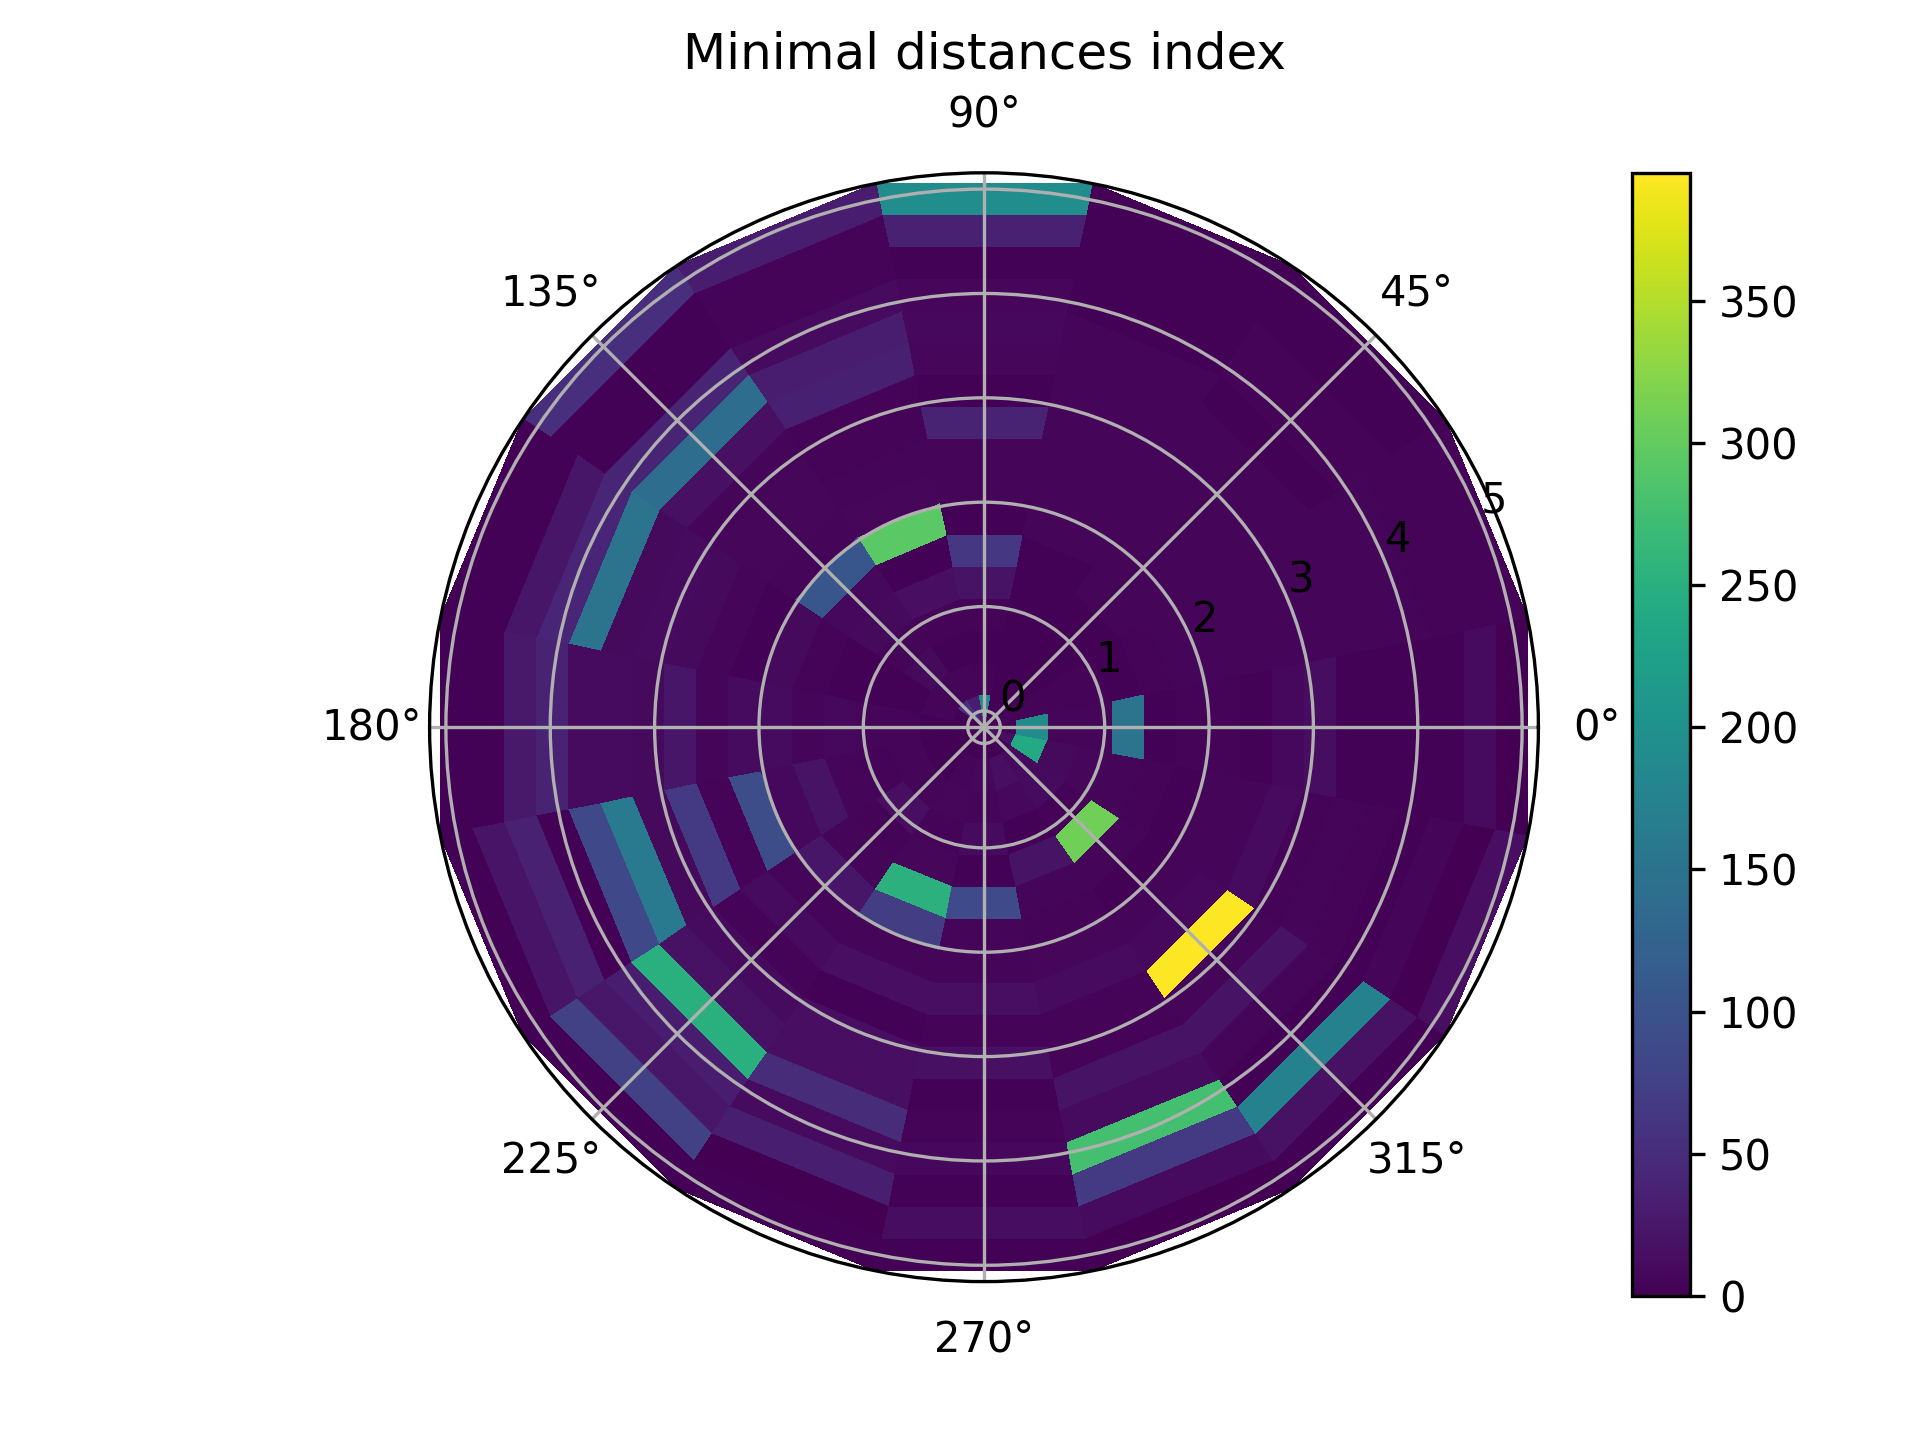
\includegraphics[width=0.31 \linewidth]{figures/experiments/Minimal_distances_index_baseline_5_1691621331_5000.png}
            \label{fig:SAC_baseline_min_distance_step/5}
            }
        \hfill
        \subfloat[$N = 10$]{
            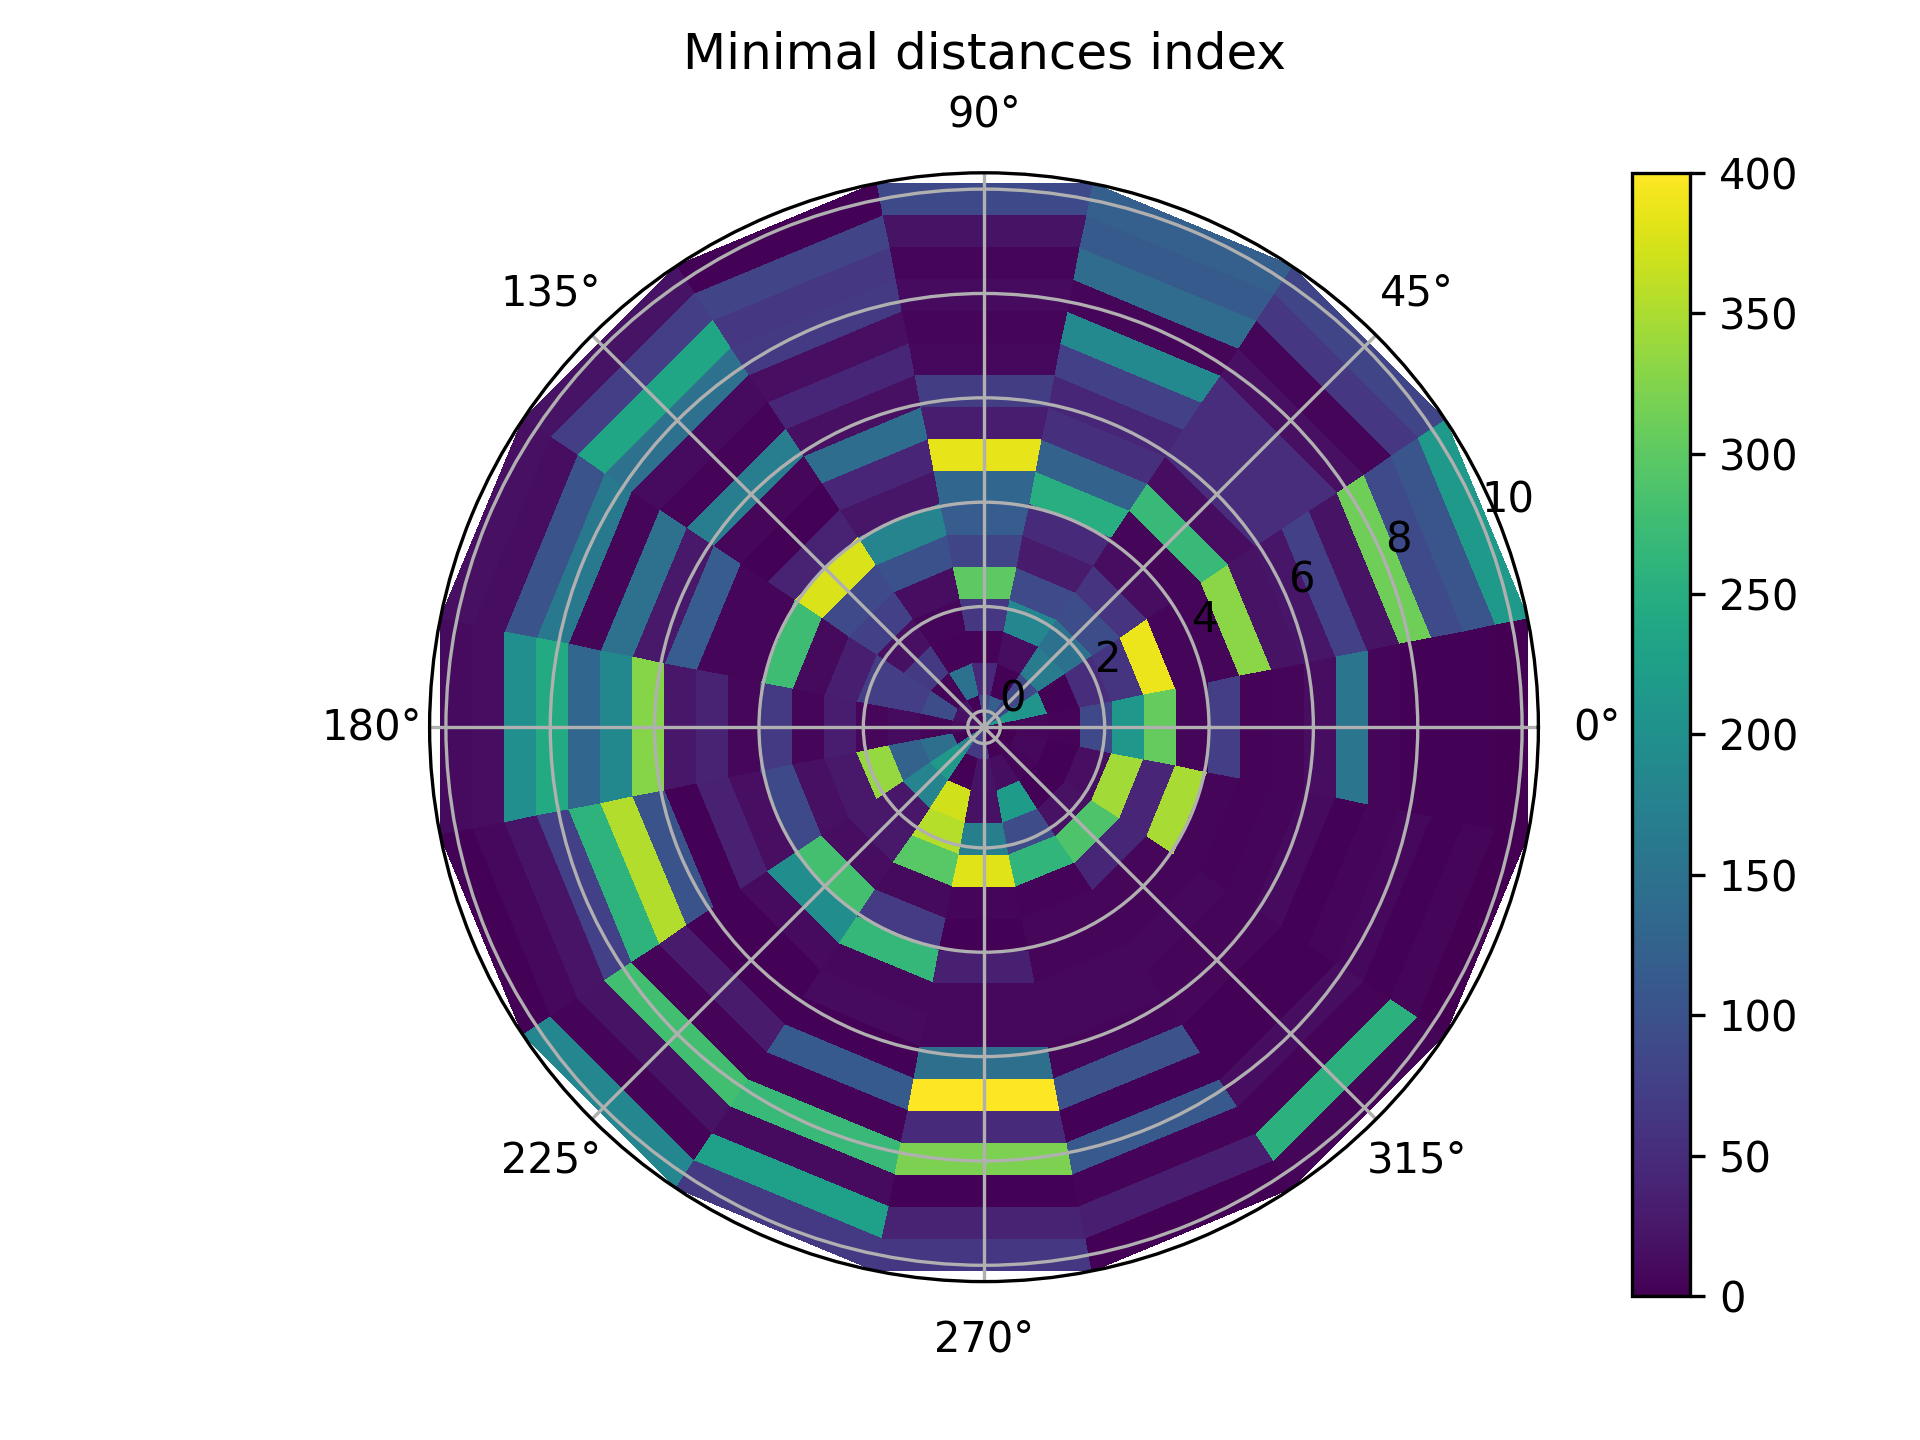
\includegraphics[width=0.31 \linewidth]{figures/experiments/Minimal_distances_index_baseline_10_1691618968_5000.png}
            \label{fig:SAC_baseline_min_distance_step/10}
            }
    \end{center}
    \caption[SAC iteration heatmap]{Heatmap of how many iterations baseline SAC has needed to solve inverse kinematics starting from $[N, 0]$ targeting the middle of each polygon. The maximum budget is 20 times $N$ with a target precision of $0.1$.}
    \label{fig:SAC_baseline_min_distance_step}
\end{figure}

\section{SAC with Latent Model}

The integration of the Latent Model into the SAC framework yielded the results showcased in \chapref{chap:experiments}. While comprehending the striking disparities in problem-solving strategies between the trained latent models, as illustrated in \figref{fig:SAC_action_correlation}, and the Inverse Kinematics solver CCD, as depicted in \figref{fig:dataset_action_correlation}, it is rather astonishing that this approach was effective. Typically, such a substantial shift in the distribution of the observation space would result in unpredictable and unworkable behavior in the predicted actions within the Action space. We attempted to address this challenge by introducing the imitation loss, emphasizing predicted actions that led to state angles much closer to the original distribution.

As seen earlier, we obtained varying performances from the VAEs with different latent dimensions. But why? Let's first consider the experiments with a latent dimension of two. Given that we are endeavoring to encode two-dimensional target information, which is sampled in accordance with the concept of the \texttt{TargetGaussianDataset}, into a two-dimensional Gaussian manifold, the most efficient strategy for retaining information would involve channeling the mean values while returning a standard deviation close to zero. Since we employ the Evidence Lower Bound (ELBO) with a Gaussian distribution for a Variational Autoencoder (VAE), we must select a parameterized latent distribution that closely approximates the standard normal distribution. An additional challenge lies in encoding the target position as independent random variables. Given these properties and constraints, compressing this information can indeed be quite challenging. On the other hand, selecting a latent dimension that is too high can introduce excessive computational complexity, sampling difficulties, and a reduction in robustness.

Based on these observations, we propose setting the latent dimension of a VAE as an additional hyperparameter to optimize. Setting it too high can result in the extremely high variance observed in the Soft Actor-Critic task, while setting it too low may lead to a loss of encoded information.

Furthermore, let's revisit the action correlation plots. As previously mentioned, these plots across all SAC experiments deviate significantly from the initial distribution, as depicted in \figref{fig:dataset_action_correlation}. However, they exhibit remarkable similarity among themselves, as illustrated in \figref{fig:SAC_action_correlation}. This is an unexpected outcome, as each model could adopt a distinct problem-solving strategy and start anew in each iteration. Conversely, activating the imitation loss in the VAE experiments and integrating this approach with SAC should ideally result in a substantial shift towards the rhombus-shaped distribution observed in Figure 5.4. However, the familiar hotspots seen in \figref{fig:dataset_action_correlation} vanish, and a new distribution emerges, characterized by the same spike at $(\pi, 0)$, as depicted in \figref{fig:SAC_action_correlation_comp/latent_4_imitation}.

% \begin{figure}[h]
%     \begin{center}
%         \subfloat[SAC baseline experiments]{
%             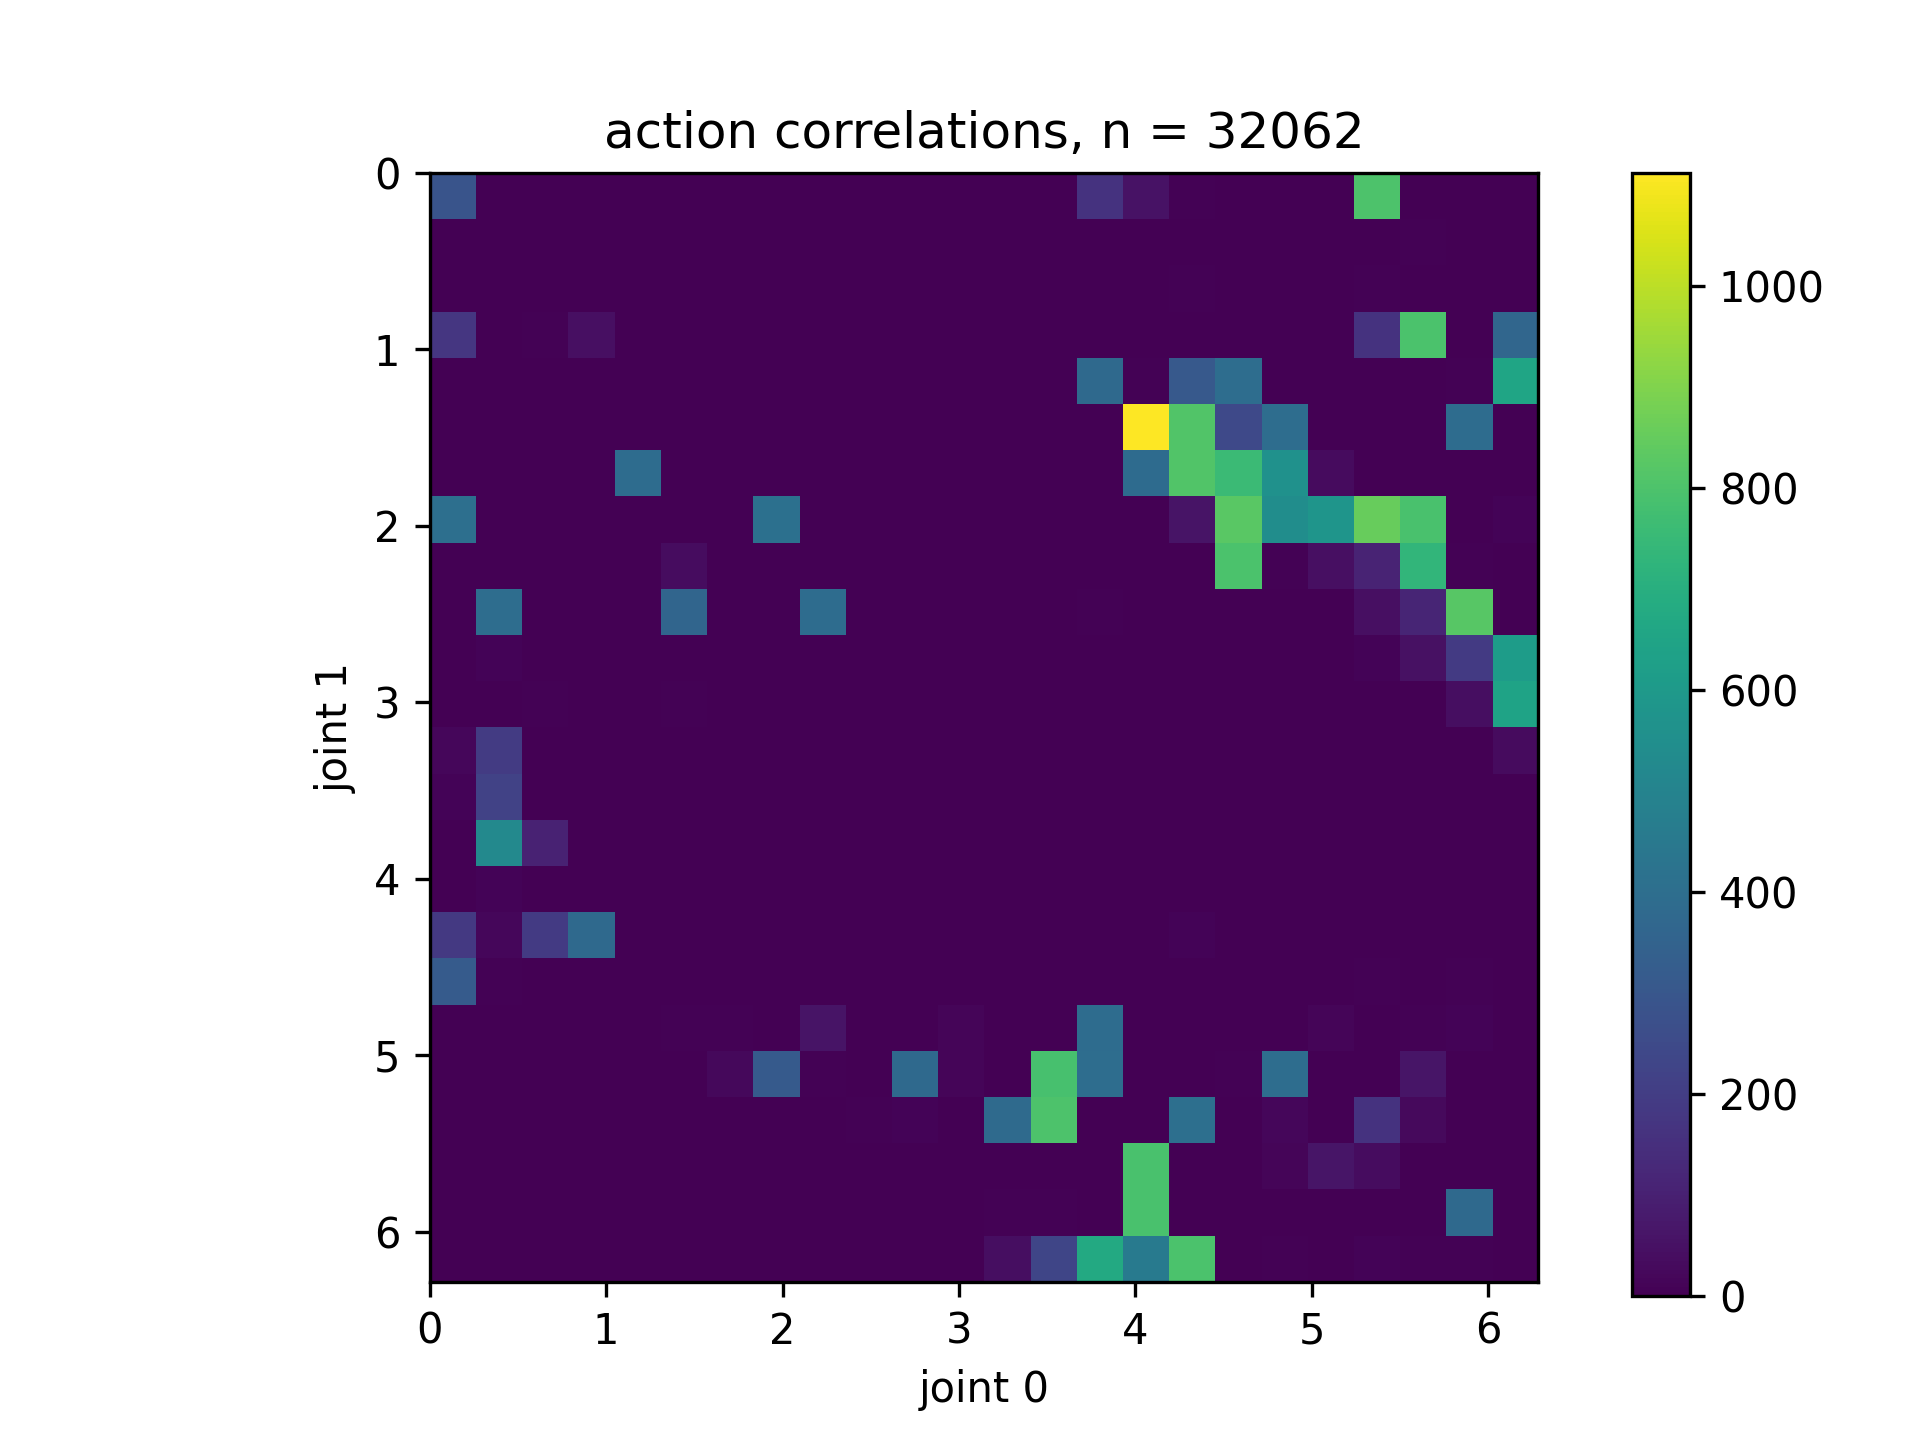
\includegraphics[width=0.31 \linewidth]{figures/experiments/action_correlations_baseline_2_1691621262_5000.png}
%             \label{fig:SAC_action_correlation_supervised/baseline}
%             }
%         \hfill
%         \subfloat[SAC + Supervised model trained only with distance loss enabled]{
%             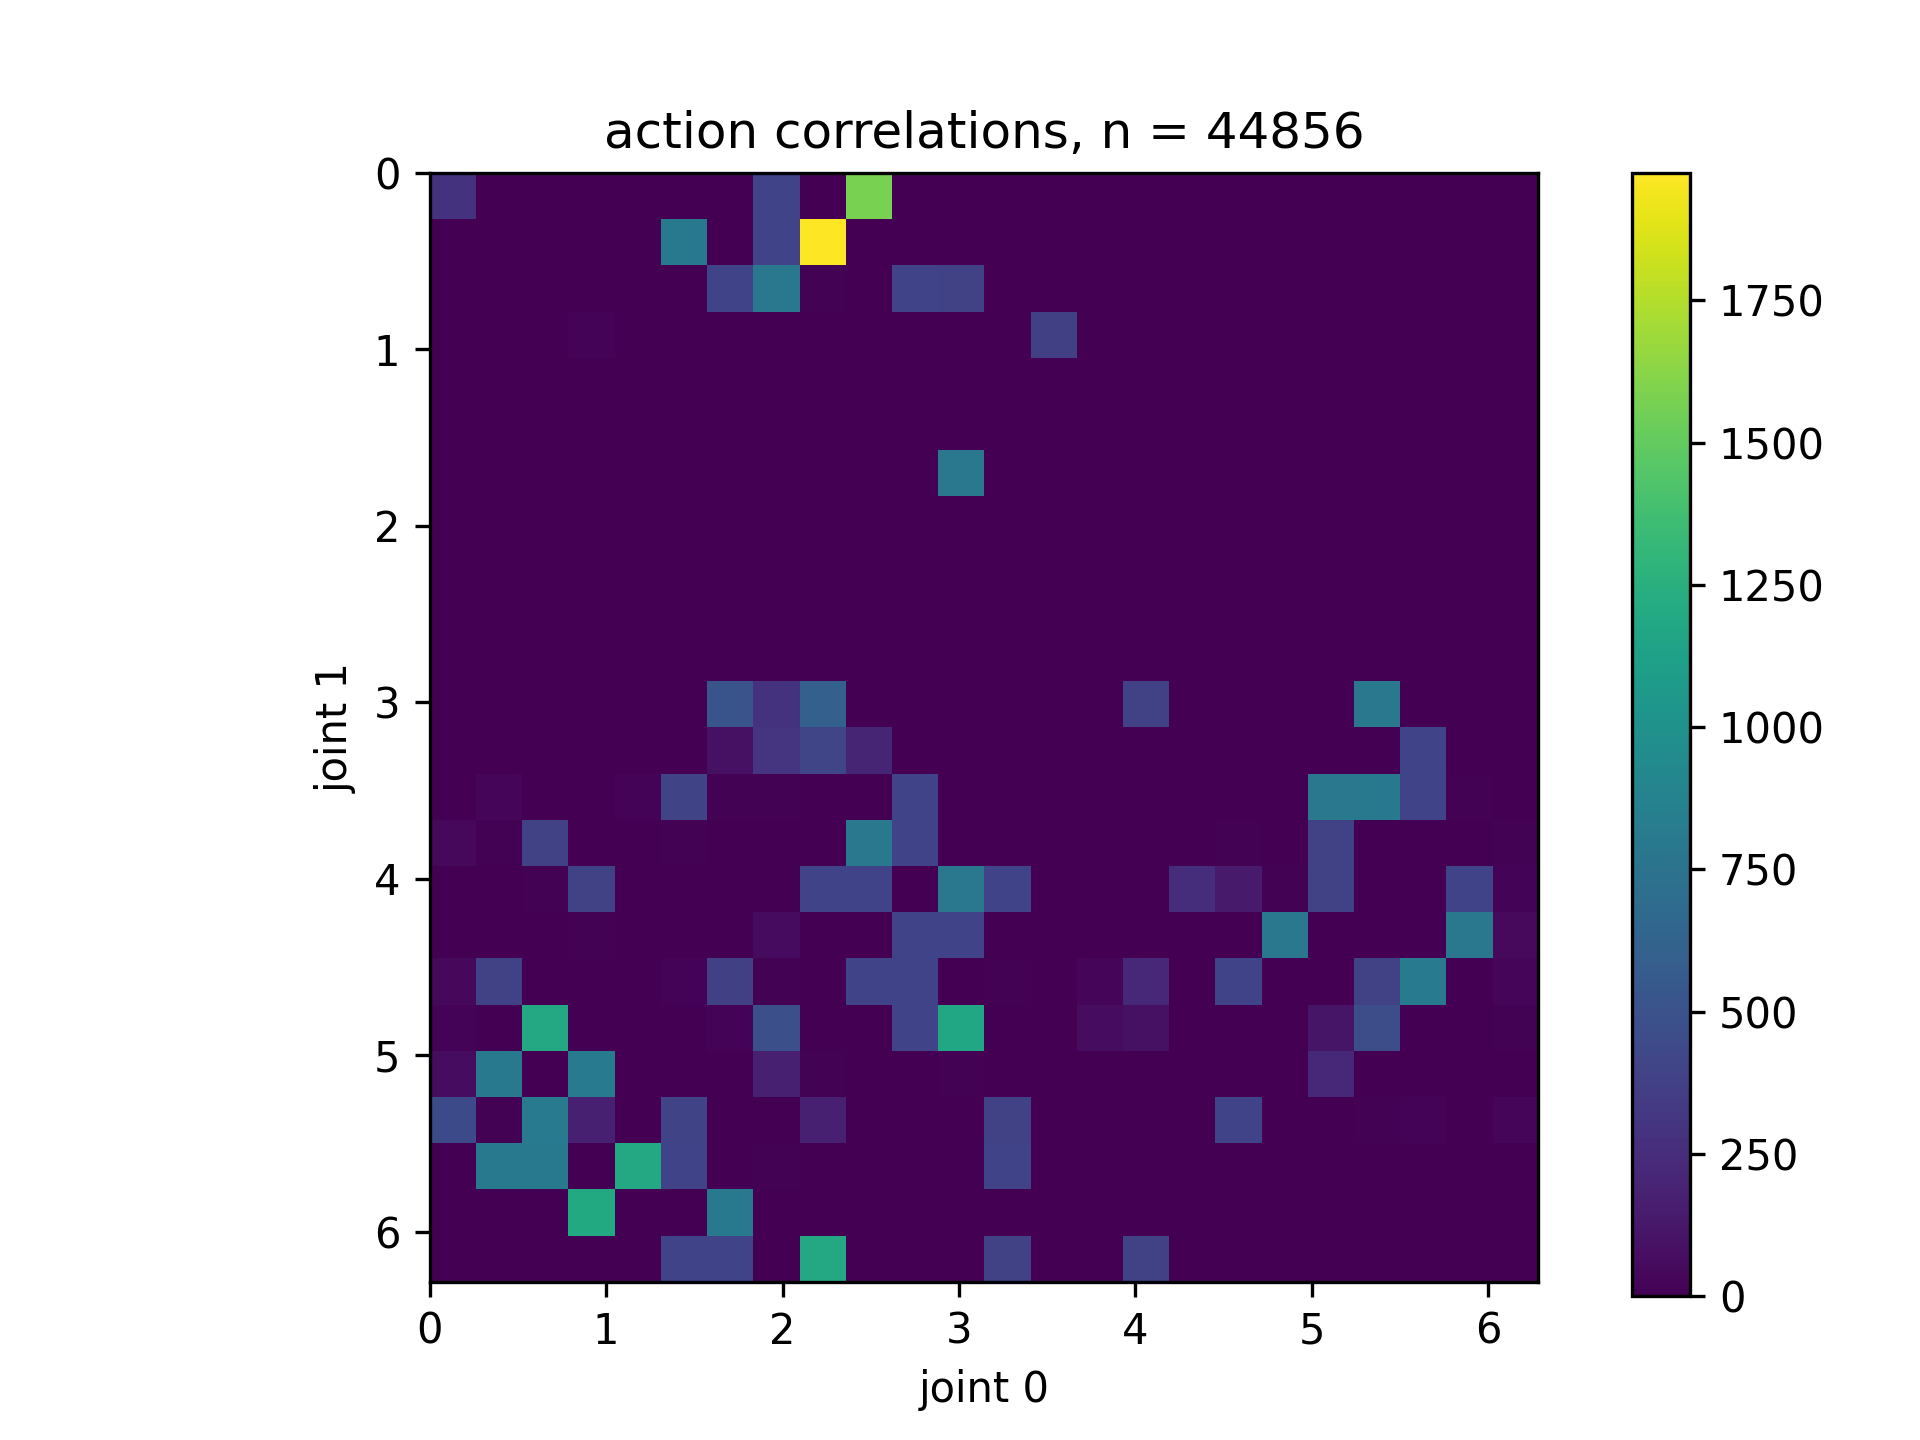
\includegraphics[width=0.31 \linewidth]{figures/experiments/action_correlations_supervised_dist_loss_2_1693272467_3000.png}
%             \label{fig:SAC_action_correlation_supervised/supervised}
%             }
%         \subfloat[SAC + Supervised model trained only with distance and imitation loss enabled]{
%             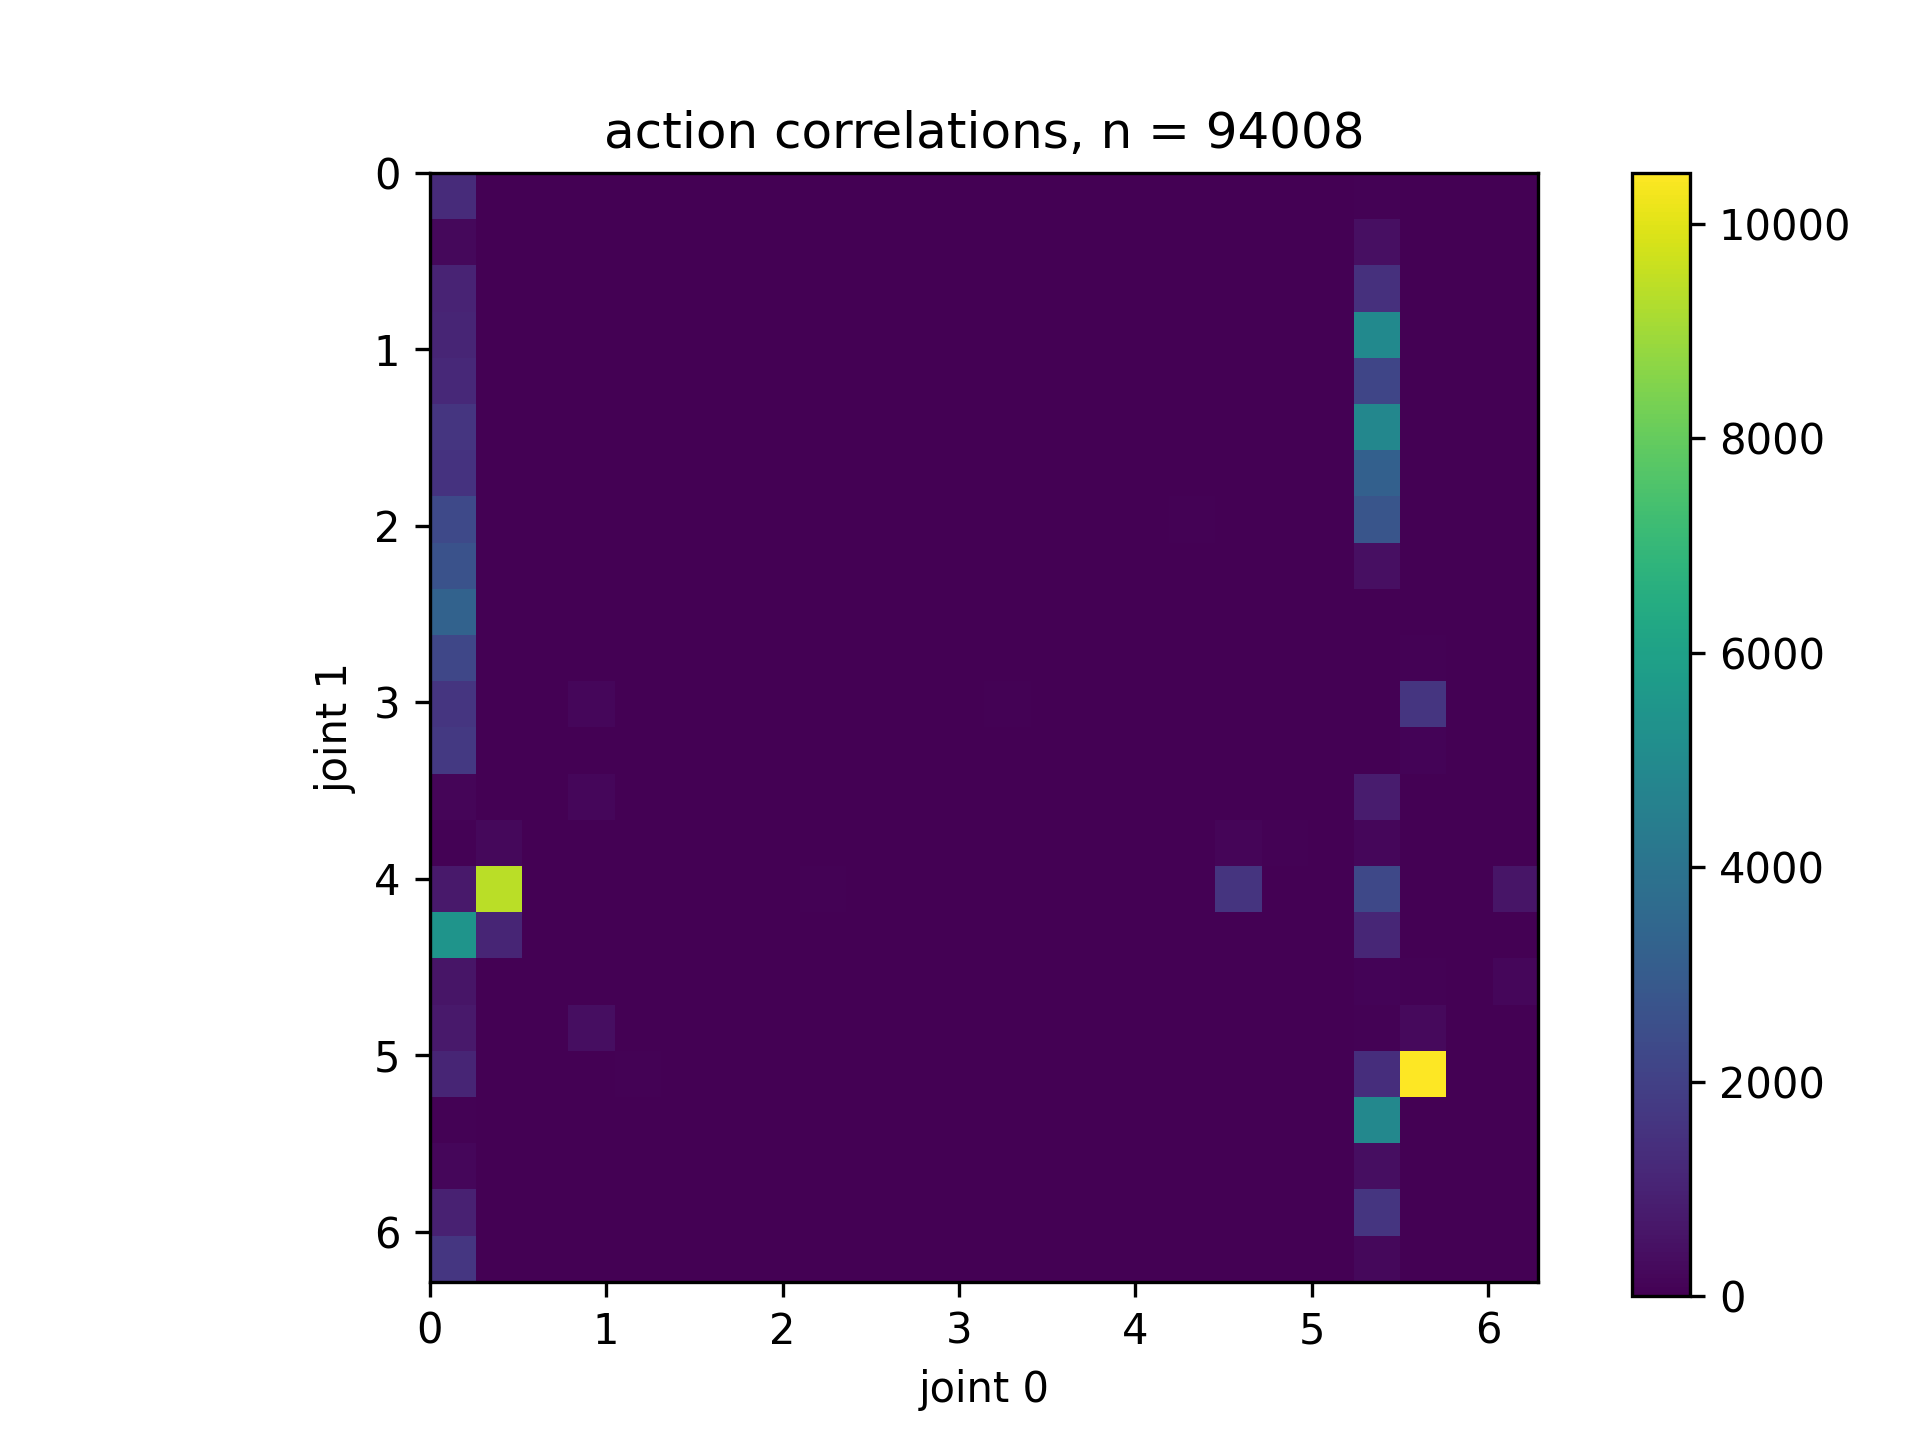
\includegraphics[width=0.31 \linewidth]{figures/experiments/action_correlations_supervised_imitation_2_1693487256_3000.png}
%             \label{fig:SAC_action_correlation_supervised/supervised_imitation}
%             }
%     \end{center}
%     \caption[action correlation comparison with supervised model]{Action correlation for baseline experiments, experiments with SAC and supervised model with only distance loss enabled and SAC with supervised model with distance and imitation loss enabled.}
%     \label{fig:SAC_action_correlation_supervised}
% \end{figure}


Finally, we want to discuss which kind of latent model someone should prefer. The VAE or the supervised learning model? \\
As we have seen in the experimental part but also in \tabref{tab:SAC_solved_ratio}, the SAC + VAE returns much more stable results and also better results compared to the supervised model. One reason might be the generalization within the training of a VAE. This results in a much smoother latent space than we could achieve with the supervised model. Another advantage of the VAE is the implied dimensionality invariance we do achieve with a constant latent dimension but a different prediction dimension. An indication for this theory can seen by the almost constant mean log probability. 


Lastly, let's address the choice between the VAE and the supervised learning model. As demonstrated in the experimental section and summarized in \tabref{tab:SAC_solved_ratio}, SAC combined with the VAE returns significantly more stable results and outperforms the supervised model. One possible reason for this is the generalization achieved within the training of a VAE. This leads to a much smoother latent space compared to what can be achieved with the supervised model. Another advantage of the VAE lies in the implied dimensionality invariance achieved with a constant latent dimension but varying prediction dimensions. This notion is supported by the nearly constant mean log probability, indicating the model's ability to capture the underlying patterns across various prediction dimensions.


\textbf{Choosing Between Latent Models}

The discussion culminates in a comparison between VAEs and supervised learning models, highlighting the advantages of each. Notably, SAC combined with VAEs returned more stable and superior results compared to the supervised model. This was attributed to the generalization capabilities inherent in VAE training, resulting in a smoother latent space compared to the supervised model. Additionally, VAEs offered dimensionality invariance with a constant latent dimension and different prediction dimensions.

Overall, the results and insights presented in this discussion section offer a valuable foundation for understanding the performance and potential applications of VAEs and supervised models in solving complex tasks like inverse kinematics in robotic systems. The choice between these models depends on specific use cases and optimization objectives.
